\documentclass[a4paper,11pt,fleqn]{mira-author}
\usepackage[numbers,sort&compress]{natbib}
\usepackage{newpxtext}
\usepackage{iftex}
\ifPDFTeX
 \usepackage{newpxmath}
\else
 \usepackage{unicode-math}
 \setmathfont{texgyrepagella-math.otf}
\fi
\usepackage{microtype}
\usepackage{tikz}
\usepackage{enumitem}
\usepackage{academicons}
\usepackage{fontawesome5}
\usepackage{lettrine}
\usepackage{tabularx}
\usepackage{multicol}
\renewcommand{\LettrineTextFont}{\normalfont}
\definecolor{ink}{HTML}{17232D}
\definecolor{muted}{HTML}{58646D}
\definecolor{papergray}{HTML}{F1F3F4}
\definecolor{academicgreen}{HTML}{266B46}
\definecolor{orcidgreen}{HTML}{A6CE39}
\definecolor{navy}{HTML}{204562}
\definecolor{linkedinblue}{HTML}{0A66C2}
\definecolor{researchteal}{HTML}{008E83}
\definecolor{referencefill}{HTML}{E3F2E9}
\definecolor{lossfill}{HTML}{E4EFFB}
\definecolor{shiftfill}{HTML}{DCEFF0}
\definecolor{jointfill}{HTML}{FFF0D4}
\definecolor{foresthead}{HTML}{245449}
\definecolor{mintfill}{HTML}{E8F3ED}
\definecolor{purplehead}{HTML}{654C83}
\definecolor{lavenderfill}{HTML}{EEE8F6}
\definecolor{lavenderlight}{HTML}{F7F3FB}
\definecolor{tealhead}{HTML}{1E6576}
\definecolor{cyanfill}{HTML}{E0F0F4}
\definecolor{cyanlight}{HTML}{F0F8FA}
\definecolor{rusthead}{HTML}{8C4E2D}
\definecolor{peachfill}{HTML}{F8E9DD}
\definecolor{peachlight}{HTML}{FCF4ED}
\definecolor{indigohead}{HTML}{3E4E7D}
\definecolor{indigofill}{HTML}{E8ECF8}
\definecolor{slatehead}{HTML}{45616E}
\definecolor{slatefill}{HTML}{E8EFF2}
\definecolor{plumhead}{HTML}{774D6B}
\definecolor{plumfill}{HTML}{F3E8EF}
\hypersetup{pdftitle={Reliability Assessment of Wi-Fi CSI-Based Activity Recognition under Environmental Shift and Structured Measurement Loss},pdfauthor={Abdessamad Bourkibate},hidelinks}
\geometry{paperwidth=210mm,paperheight=297mm,top=17mm,bottom=17mm,left=18mm,right=18mm,columnsep=7mm}
\setlength{\parindent}{1em}
\setlength{\parskip}{2pt}
\setlist[enumerate]{leftmargin=1.35em,itemsep=2pt,topsep=4pt,parsep=0pt}
\setlist[itemize]{leftmargin=1.2em,itemsep=2pt,topsep=4pt,parsep=0pt}
\makeatletter
\renewcommand\section{\@startsection{section}{1}{0pt}{8pt plus 2pt minus 1pt}{4pt}{\normalfont\fontsize{11.5}{14}\selectfont\bfseries}}
\renewcommand\subsection{\@startsection{subsection}{2}{0pt}{6pt plus 1pt minus 1pt}{3pt}{\normalfont\fontsize{10.5}{13}\selectfont\bfseries}}
\makeatother


% Caption spacing is explicit so full-width figures remain readable.
\setlength{\dbltextfloatsep}{18pt plus 3pt minus 2pt}
\setlength{\dblfloatsep}{20pt plus 3pt minus 2pt}
\setlength{\textfloatsep}{16pt plus 3pt minus 2pt}
\setlength{\intextsep}{14pt plus 2pt minus 2pt}
\makeatletter
\setlength{\@fptop}{0pt}
\setlength{\@fpsep}{18pt}
\setlength{\@fpbot}{0pt plus 1fil}
\setlength{\@dblfptop}{0pt}
\setlength{\@dblfpsep}{18pt}
\setlength{\@dblfpbot}{0pt plus 1fil}
\makeatother
\emergencystretch=1.5em
\hyphenpenalty=4000
\exhyphenpenalty=2000
\ExplSyntaxOn
\cs_set_protected:Npn \__make_fig_caption:nn #1#2
 {
  \par\vspace{8pt}
  \noindent\parbox{\linewidth}
   {\normalfont\fontsize{9.5}{12.5}\selectfont\raggedright
    \textbf{#1.}~#2\par}
  \par\vspace{5pt}
 }
\ExplSyntaxOff

\raggedbottom
\setcounter{topnumber}{3}
\setcounter{dbltopnumber}{3}
\setcounter{totalnumber}{5}
\renewcommand{\topfraction}{.9}
\renewcommand{\dbltopfraction}{.9}
\renewcommand{\textfraction}{.08}
% Load once in the document preamble; xcolor[table], array/tabularx required.
\definecolor{m2head}{HTML}{204562}
\definecolor{m2border}{HTML}{536F80}
\definecolor{m2Afill}{HTML}{E8EFF4}
\definecolor{m2Bfill}{HTML}{EDF1F3}
\definecolor{m2Cfill}{HTML}{F0ECF6}
\definecolor{m2Dfill}{HTML}{F9EEE6}
\definecolor{m2Efill}{HTML}{E6F4F1}
\definecolor{m2Elight}{HTML}{F1F9F7}
\definecolor{m2Ehead}{HTML}{007F76}
\providecommand{\mTwoHead}[1]{\textcolor{white}{\strut\bfseries #1}}

\definecolor{mrefHead}{HTML}{204562}
\definecolor{mrefBorder}{HTML}{536F80}
\definecolor{mrefE}{HTML}{E6F4F1}
\definecolor{mrefMR}{HTML}{F0ECF6}
\definecolor{mrefA}{HTML}{E8EFF4}
\definecolor{mrefB}{HTML}{EDF1F3}
\providecommand{\mrefHeadText}[1]{\textcolor{white}{\strut\bfseries #1}}

\makeatletter
\def\ps@authorpages{%
 \def\@oddhead{}\def\@evenhead{}%
 \def\@oddfoot{\hfil{\normalfont\fontsize{8.5}{10}\selectfont\thepage}\hfil}%
 \let\@evenfoot\@oddfoot}
\makeatother

\begin{document}
\pagestyle{authorpages}
\color{ink}
\twocolumn[{
\begin{minipage}{\textwidth}
{\sffamily\fontsize{8}{10}\selectfont\color{muted}RESEARCH MANUSCRIPT \textbullet{} NOT PEER REVIEWED\hfill 28 October 2026\par}
\vspace{3mm}
{\fontsize{18}{21}\selectfont\bfseries\centering Reliability Assessment of Wi-Fi CSI-Based Activity Recognition\\under Environmental Shift and Structured Measurement Loss\par}
\vspace{2mm}
{\fontsize{10.5}{13}\selectfont\itshape\centering A participant-disjoint study of joint environment--cohort transfer and post-normalization observation loss.\par}
\vspace{4mm}
\begingroup\centering
{\fontsize{14}{16}\selectfont\bfseries\href{https://orcid.org/0009-0000-6186-8071}{Eng. Abdessamad Bourkibate}\par}
\vspace{1mm}
{\fontsize{13}{15}\selectfont
\href{https://orcid.org/0009-0000-6186-8071}{\textcolor{orcidgreen}{\aiOrcid}}\hspace{5mm}
\href{https://github.com/ABDESSAMAD-BOURKIBATE}{\textcolor{navy}{\faGithub}}\hspace{5mm}
\href{https://www.linkedin.com/in/abdessamad-bourkibate-b17717350/}{\textcolor{linkedinblue}{\faLinkedin}}\hspace{5mm}
\href{https://www.researchgate.net/profile/Abdessamad-Bourkibate-2}{\textcolor{researchteal}{\aiResearchGate}}\par}
\vspace{1.5mm}
{\fontsize{10.5}{13}\selectfont Software \& Cybersecurity Engineer \textbar{} AI \& EdTech\par}
{\fontsize{10.5}{13}\selectfont Share'In Holding\par}
\vspace{1mm}
{\sffamily\fontsize{9.2}{11.5}\selectfont
\href{mailto:a.bourkibate@share-in.ma}{\textcolor{navy}{\faEnvelope\;a.bourkibate@share-in.ma}}\par}
\endgroup
\vspace{4mm}
{\fontsize{11}{13}\selectfont\bfseries Abstract\par}
\vspace{1mm}
{\fontsize{10}{12.3}\selectfont
Wi-Fi channel state information (CSI) supports contactless activity recognition, but performance in one acquisition setting does not establish reliability after environmental change and measurement loss. We evaluate 1,260 genuine recordings from 30 participants in three indoor environments using participant-disjoint source partitions and leave-one-environment-out tests. An initial 60-fit model comparison and a separate 90-fit component-removal study retain mixed and adverse results for compact missingness-informed and residual networks. A further exploratory execution freezes 75 source-fitted models across five prespecified configurations before their test evaluation. Fixed log-mean-power inputs feed observed-endpoint temporal moments and generalized covariance spectra. The declared feature-only MLP arm E achieves mean held accuracy of $75.17\pm1.00$\% on complete input, $73.82\pm0.94$\% with random 50\% loss, and $60.60\pm1.37$\% with contiguous 50\% loss. These deviations describe five training seeds after within-seed mask averaging. Its contiguous-loss macro F1 is 59.16\%; two seed accuracies remain below 60\%. The primary matched-endpoint versus observed-cell normalization contrast in the hybrid model is only $+0.54\pm0.65$ macro-F1 percentage points. E's result therefore does not establish that support matching alone causes the improvement. Source-only calibration, recognition, proper probability scores and repeated-view dependence are documented alongside verified checkpoints and saved predictions. An additional fixed-power-input MiniRocket reference reaches 53.84\% complete and 19.41\% contiguous-loss accuracy. Its clean-source training and mean filling differ from E's loss augmentation and observed-mask features; this comparison does not isolate architecture. Different cohorts occupy each environment, and missingness is simulated after packet-index normalization. Historical target outcomes influenced development; external replication and matched controls are needed before general performance or deployment claims.\par}
\vspace{2mm}
{\sffamily\fontsize{8.7}{11}\selectfont\textbf{Keywords:} Wi-Fi sensing; channel state information; activity recognition; environmental shift; missing measurements; predictive reliability.\par}
\vspace{3mm}
\end{minipage}
}]
\fontsize{10.5}{13}\selectfont

\section{Introduction}
\lettrine[lines=3,lhang=0,loversize=.08,findent=.45em,nindent=0pt]{\color{academicgreen}W}{i-Fi} networks provide an existing medium for contactless sensing in homes, classrooms, and workplaces. Human motion perturbs multipath propagation, and these perturbations can be represented through channel state information (CSI). Learning-based systems can use this representation to infer activity without a camera or a body-worn device \cite{zinys2021,guarino2026}. Their usefulness depends on understanding how predictions behave when the sensing conditions depart from those represented in the training data.

Two sources of variation merit joint attention. The first is \emph{environmental shift}: changes in room geometry, furniture, or sensor placement alter the propagation paths encoded in CSI \cite{zinys2021}. The second is \emph{structured measurement loss}, where consecutive observations are unavailable. When these conditions occur together, both recognition performance and the confidence attached to a decision may change. A plausible activity label and a high predicted probability can therefore provide an incomplete account of reliability.

Domain adaptation has been investigated as a means of reducing sensitivity to changing domains \cite{zinys2021}. A recent review also identifies environmental robustness, consistent evaluation, and reproducibility as continuing challenges \cite{guarino2026}. These findings motivate a controlled assessment of how measurement availability interacts with environmental shift.



\begin{figure*}[t]
\centering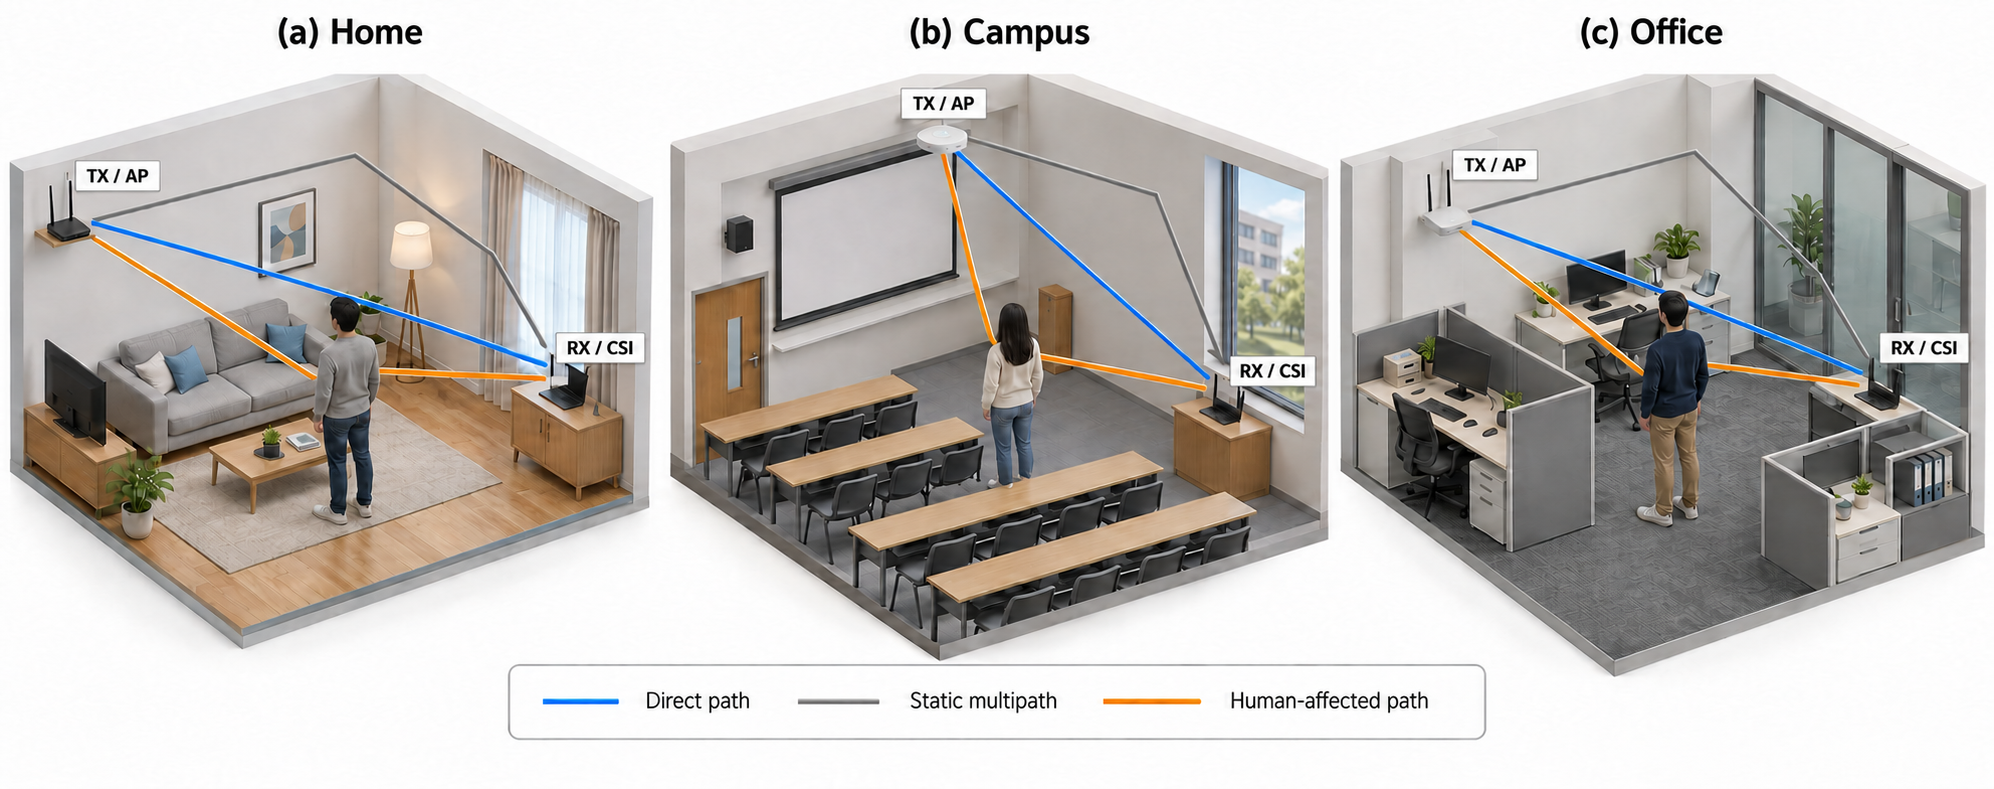
\includegraphics[width=.96\textwidth]{deployment-contexts.png}
\caption{Illustrative home, university Campus, and office geometries. Blue identifies a selected direct path, gray selected static multipath, and amber a selected human-affected contribution. TX/AP sends and RX/CSI samples the combined channel. These explanatory scenes are not measured study sites or a ray-tracing solution.}
\label{fig:contexts}
\end{figure*}

\section{Related work}
Zinys et al. study domain-independent activity recognition using a generative adversarial network and simplified CSI preprocessing \cite{zinys2021}. Their work addresses sensitivity to changes in sensing conditions. It provides a relevant robustness baseline, but reported accuracies cannot be transferred to a different dataset, split, or degradation model.

DensePose From WiFi maps signal phase and amplitude to dense body-surface coordinates across 24 human regions \cite{geng2022}. This is a spatial reconstruction task, whereas the present study predicts discrete activity labels. Dense pose estimates do not establish that a generic router can measure physiological signals or reproduce those results in every room. The preprint is therefore background on sensing capability, rather than a directly comparable activity classifier.

Widar3.0 estimates body-coordinate velocity profiles to reduce dependence on environment, position, and orientation \cite{zheng2019}. Its central insight is that a physically informed representation can suppress domain-specific signal variation. This motivates evaluating robustness across explicit domain partitions, while distinguishing gesture recognition from whole-body activity recognition.

SenseFi provides a common implementation and benchmark for several Wi-Fi sensing datasets and learning architectures \cite{yang2023}. The authors describe UT-HAR as a single-environment dataset whose sliding-window samples can overlap. They also describe NTU-Fi HAR recordings from three layouts. These distinctions matter: random sample splits and environment-held-out splits answer different questions. Dataset identity alone does not establish that a processed release preserves the metadata needed for an independent cross-environment evaluation.

Learned handling of incomplete CSI predates the present implementation. CSI-BERT reconstructs missing CSI using self-supervised bidirectional representations \cite{zhao2024csibert}; CSI-BERT2 extends pretraining and fine-tuning to CSI prediction and classification with temporal embeddings and adaptive subcarrier re-weighting \cite{zhao2026csibert2}. Zakeri et al. encode the age of retained samples relative to the session decision and fuse it with CSI embeddings \cite{zakeri2026age}. These approaches establish prior work on missingness and temporal context. Their reported performance is not a matched baseline here, because datasets, acquisition assumptions, training access and tasks differ.

Guarino et al. examine the availability of datasets, preprocessing descriptions, and code needed to reproduce CSI sensing studies \cite{guarino2026}. Their analysis motivates retaining file-level provenance, domain identifiers, and complete evaluation settings. We document the releases actually used and audit their sampling units before interpreting performance.

Guo et al. distinguish classification accuracy from probability calibration and evaluate post-hoc temperature scaling \cite{guo2017}. Their empirical findings concern the evaluated neural networks and datasets; they do not establish that calibration will survive CSI degradation. Here, calibration parameters are fitted using source validation observations only and frozen before test evaluation.

Geifman and El-Yaniv frame selective classification as a trade-off between prediction risk and coverage \cite{geifman2017}. Following this distinction, a model that accepts fewer observations must be compared at a matched acceptance rate. We compute full-coverage recognition alongside confidence-ranked selective error; rejection alone is not interpreted as improved recognition. Distribution shift also requires separate assessment; a risk guarantee proved under specific assumptions will not be imported into this evaluation without checking those assumptions.

The experiment combines an environment factor with a measurement-availability factor. Random masks and contiguous missing blocks are compared at matched missing fractions using the same test recordings and frozen models. Masks are controlled corruptions of genuine recordings, not observed network outages.

Alsaify et al. provide recordings with explicit environment, subject, experiment, activity, and trial identifiers \cite{alsaify2020}. Their author repository also supplies parsed MAT files and amplitude-scaling code \cite{multienvdata}. These labels permit environment exclusion and participant-disjoint partitions. The three environments contain different participant cohorts, which limits causal interpretation of the environmental comparison.

Our contribution is a reproducible reliability evaluation of this combined transfer and measurement-loss setting. It includes recognition, probability quality, class errors, and conditional participant-grouped uncertainty. It is an evaluation of fixed accessible baselines, rather than a claim of a new pose-reconstruction architecture or a best-performing classifier.

\section{Propagation and measurement}
Wi-Fi sensing observes a communication channel. A transmitter emits radio signals and a compatible receiver estimates how propagation changes their amplitude and phase across subcarriers and antenna links. This channel state information is more detailed than a single received-power indicator. Halperin et al. describe a practical interface for collecting such measurements from a supported wireless card \cite{halperin2011}. The channel estimate is the input to an inference procedure; it does not itself contain an anatomical image.

An explanatory multipath model for subcarrier $k$ and antenna link $r$ is
\begin{equation}
\widehat H_{k,r}(t)=\sum_{p=1}^{P}a_{p,r}(t)
 e^{-j2\pi f_k\tau_{p,r}(t)}+\eta_{k,r}(t),
\label{eq:channel}
\end{equation}
where $a_{p,r}$ is the complex coefficient of path $p$, $\tau_{p,r}$ is its delay, and $\eta_{k,r}$ collects noise and residual measurement effects. This simplified representation explains superposition, rather than solving the electromagnetic field in the illustrated rooms. Practical CSI also contains hardware timing and phase effects that must be considered during preprocessing \cite{guarino2026}.

The received signal combines relatively direct contributions with paths affected by walls, furniture, and people. Body movement can change path length, attenuation, and scattering. Their complex sum can increase or decrease even when the person's movement is smooth. For a change in a path's propagation length $\Delta L_p$, the corresponding phase change is approximately
\begin{equation}
\Delta\varphi_p=-2\pi\Delta L_p/\lambda,
\end{equation}
where $\lambda$ is wavelength. This sensitivity to geometry motivates temporal and physically informed features, including the body-coordinate velocity profiles studied in Widar3.0 \cite{zheng2019}.

\begin{figure*}[t]
\centering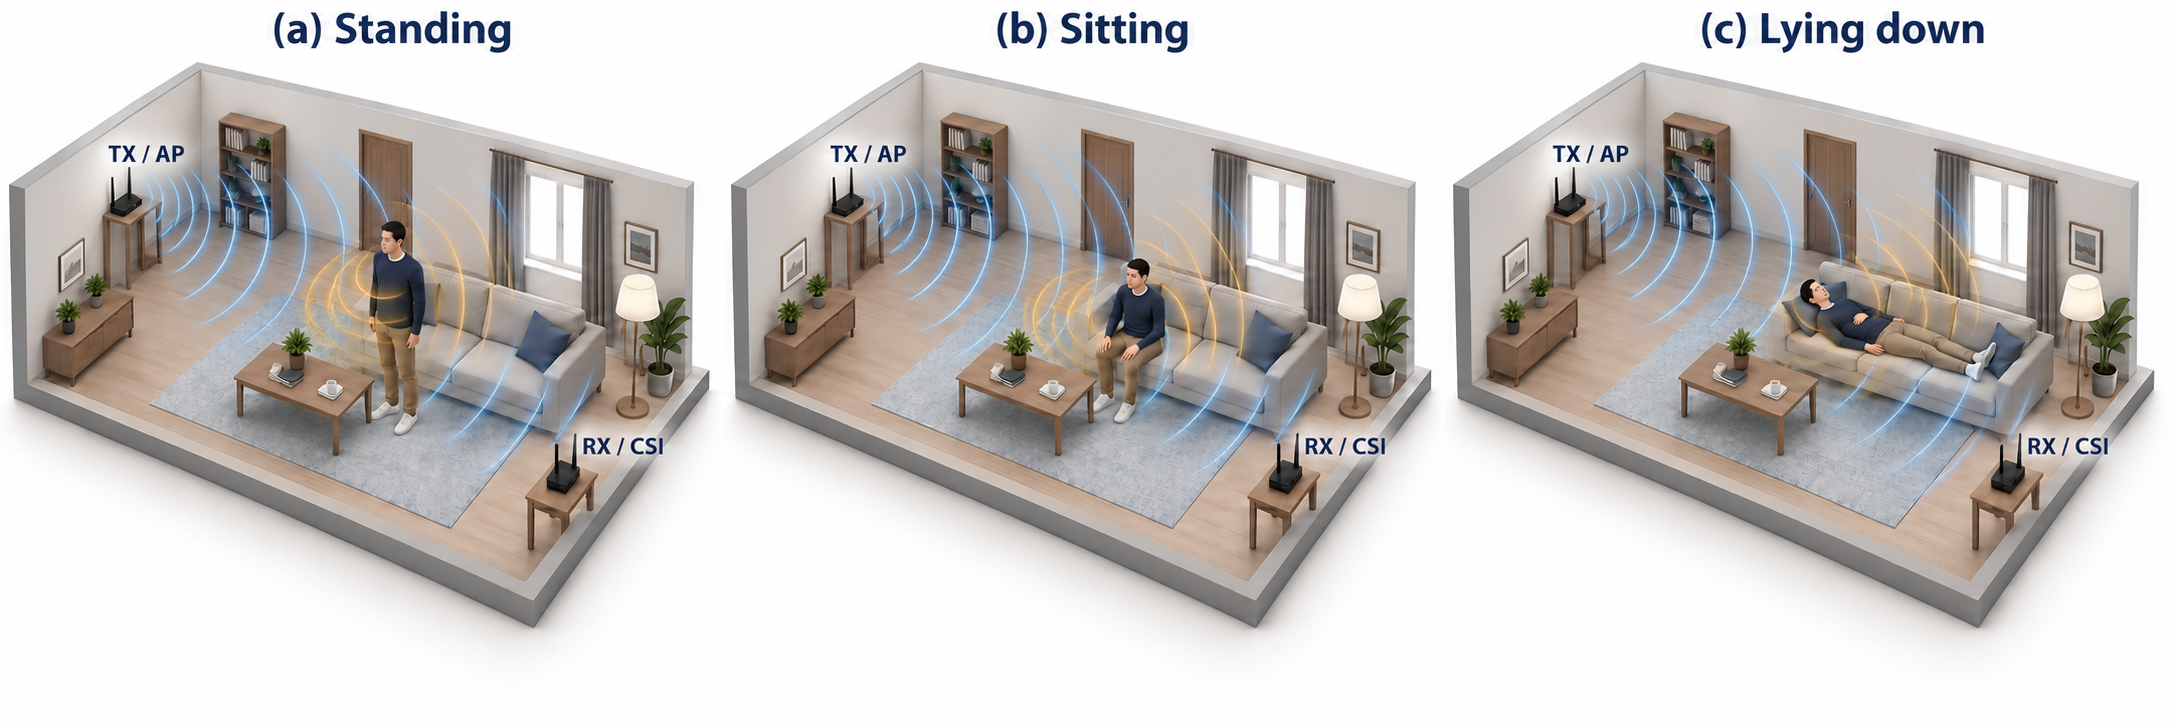
\includegraphics[width=.96\textwidth]{posture-wavefronts.png}
\caption{Fixed-room comparison of standing, sitting, and lying. Blue arcs represent illustrative incident wavefronts; amber arcs represent illustrative body-scattered contributions. Arc spacing and magnitude are not to scale or computed by a wave solver. These illustrative postures explain geometry and are not classes evaluated by the six-activity pilot.}
\label{fig:postures}
\end{figure*}

For a single moving scatterer and stationary transmitter and receiver, differentiating the path phase gives the instantaneous Doppler contribution
\begin{equation}
 f_{D,p}=\frac{1}{2\pi}\frac{d\varphi_p}{dt}
 =-\frac{1}{\lambda}\frac{dL_p}{dt}
 =-\frac{\mathbf v\!\cdot\!(\mathbf u_T+\mathbf u_R)}{\lambda}.
\label{eq:doppler}
\end{equation}
Here $\mathbf v$ is scatterer velocity, and $\mathbf u_T$ and $\mathbf u_R$ point from the transmitter and receiver, respectively, toward that scatterer. This is a bistatic single-bounce geometric relation; multiple body segments contribute different path changes. It explains motion sensitivity, but does not provide a unique inversion from CSI to human pose. The present experiment uses amplitudes only and does not estimate Doppler or recover calibrated phase.

The colors in Figures~\ref{fig:contexts} and \ref{fig:postures} have explicit explanatory roles. Blue identifies a selected transmitted or direct contribution, amber identifies a human-affected contribution, and gray identifies selected reflections involving static surroundings. They do not encode measured strength, distinct frequency bands, or recognition confidence. The person scatters and attenuates the incident field; the amber contribution does not imply that the person actively emits a Wi-Fi signal.

The arcs schematize cross-sections of wavefronts, meaning equal-phase locations of an idealized contribution. They are drawn widely apart for legibility. Radio propagation fills a volume, and the receiver samples the superposed field rather than a sequence of narrow rays scanning anatomical landmarks. A standing torso, bent seated limbs, and a horizontal body change the geometry differently. However, different combinations of position, furniture, and posture can produce similar observations. A reliable classifier must be tested on the variations it is intended to handle.


Water content provides physiological context for body--wave interaction. The often quoted 60\% refers to an illustrative whole-body mass fraction, not a universal constant or a measured value for the participants in this dataset. The USGS describes adult body water as up to about 60\% and notes variation with age and body composition \cite{usgs2019}. Water is distributed within tissues rather than pooled in a separate compartment shaped like part of the silhouette.

\begin{figure*}[t]
\centering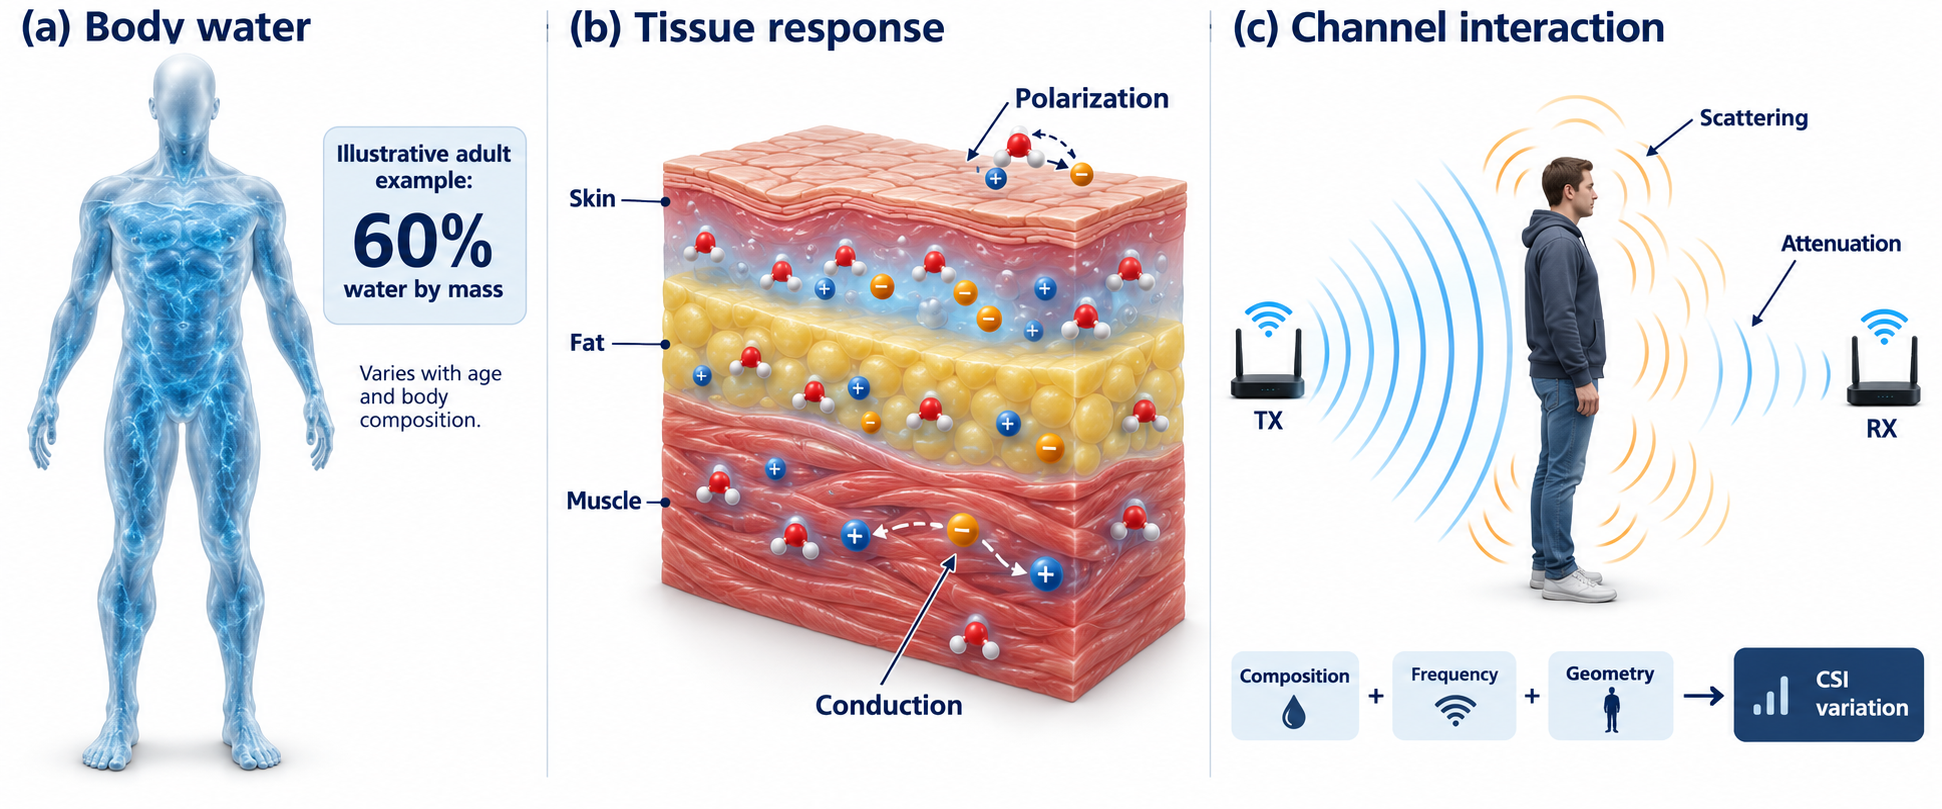
\includegraphics[width=.96\textwidth]{tissue-water-interaction.png}
\caption{Body water, tissue response, and channel interaction. The 60\% badge is a qualified illustrative adult mass fraction \cite{usgs2019}, not a measurement of a study participant. Tissue layers, molecules, ions, and wavefronts are schematic and not to scale; icon counts do not encode concentrations. Water and ions contribute to dielectric response, while frequency and geometry also determine propagation \cite{gabriel1996}. This explanatory figure does not estimate hydration or depict a measured RF field.}
\label{fig:water}
\end{figure*}

For radio propagation, the relevant material description is frequency-dependent dielectric response. Water polarization and mobile ions contribute to the response of heterogeneous biological tissues, whose properties differ by tissue type. Gabriel and Gabriel report tissue measurements and dispersion modelling over broad RF and microwave frequency ranges \cite{gabriel1996}. An effective complex relative permittivity can be written, using the $e^{j\omega t}$ convention, as
\begin{equation}
\epsilon_r^*(\omega)=\epsilon_r'(\omega)
 -j\frac{\sigma_{\mathrm{eff}}(\omega)}{\omega\epsilon_0},
\end{equation}
where $\epsilon_r'$ describes the real part and $\sigma_{\mathrm{eff}}$ combines effective loss mechanisms in this representation. These quantities influence phase and attenuation; interfaces, incidence direction, polarization, and body geometry also affect scattering. The whole-body water fraction cannot be substituted for a tissue permittivity or converted directly into an activity label.

Figure~\ref{fig:water} therefore links composition to a material response and then to propagation. Neither experiment measures body water or tissue dielectric properties. Observed CSI variations cannot be interpreted as hydration estimates, temperatures, or subject-specific water percentages.



The inference pipeline separates radio observations from an estimated activity or rendered human representation. A receiver first exports CSI observations. Preprocessing aligns the time series, handles missing samples, and constructs input features. A trained model then estimates an output defined by its supervision. The present study returns one of seven activity labels and a probability vector. DensePose From WiFi instead estimates body-surface correspondence \cite{geng2022}. A green wireframe body is therefore a representation of a different inference target, not a physical shape formed by radio waves in the room. 



Deployment context changes the inference problem. In a home, moving the sofa or the access point changes background propagation. A campus classroom adds different dimensions, desk arrangements, and potentially several moving occupants. In an office, partitions and occupancy patterns introduce further channel variation. These factors motivate separate environment and occupancy evaluations rather than transferring a single-room score to other buildings \cite{guarino2026}.

The word \emph{Campus} identifies a university context or a possible network name. An SSID does not specify a CSI export interface or enable sensing by itself. Acquisition needs a compatible radio, suitable firmware or driver access, packets to observe, and a defined receiver configuration. Espressif's documentation, for example, specifies explicit CSI configuration and a reception callback on supported ESP32 platforms \cite{espressif2026}. Such support establishes how to acquire measurements. Recognition of human activity still requires a trained model, appropriate labels, and validation in the intended environment.




\section{Experimental design}
This study tests how activity recognition and predictive confidence change under environment-and-cohort transfer together with structured measurement loss. Familiar-environment tests also exclude training participants, so the comparison does not rely on recognizing people observed during fitting.

\begin{center}
\begin{minipage}{\columnwidth}
\refstepcounter{table}\label{tab:design}
{\fontsize{9.3}{12}\selectfont\textbf{Table~\thetable.} Evaluated conditions by domain.\par}
\vspace{5pt}
\begingroup
\sffamily\fontsize{9.2}{12}\selectfont
\setlength{\tabcolsep}{5pt}
\renewcommand{\arraystretch}{1.45}
\renewcommand{\tabularxcolumn}[1]{m{#1}}
\begin{tabularx}{\linewidth}{>{\raggedright\arraybackslash}m{.36\linewidth}*{2}{>{\centering\arraybackslash}X}}
\rowcolor{navy}
\multicolumn{1}{l}{\textcolor{white}{\bfseries CSI input}} & \multicolumn{1}{c}{\textcolor{white}{\bfseries Familiar}} & \multicolumn{1}{c}{\textcolor{white}{\bfseries Held-out}}\\
\cellcolor{papergray}Complete & \cellcolor{referencefill}Reference & \cellcolor{shiftfill}Transfer\\
\cellcolor{papergray}Random loss & \cellcolor{lossfill}Loss only & \cellcolor{jointfill}Joint\\
\cellcolor{papergray}Contiguous loss & \cellcolor{lossfill}Loss only & \cellcolor{jointfill}Joint\\
\end{tabularx}
\endgroup
\par\vspace{5pt}
{\fontsize{8.2}{10.3}\selectfont\color{muted}Colour denotes test conditions, not accuracy.\par}
\end{minipage}
\end{center}

\noindent The initial evaluation has three parts:
\begin{enumerate}
\item quantify separate and combined degradation;
\item compare recognition and probability quality; and
\item retain reproducible splits, settings, and predictions.
\end{enumerate}




\section{Mathematical formulation}
Let $X\in\mathbb R^{C\times500}$ denote a fixed-length representation of one recording. The measured channel has $C=90$ scaled log-amplitude coefficients, reduced to 18 five-subcarrier bands for the implemented learning pipelines. A binary temporal mask $m_t$ is shared by every channel: $m_t=1$ denotes an observed time position and $m_t=0$ a missing one. Its missing fraction is
\begin{equation}
 q=1-\frac{1}{500}\sum_{t=1}^{500}m_t.
\label{eq:mask}
\end{equation}
Missing entries are treated as unavailable, rather than as physical zero-amplitude measurements. For observed indices $a<t<b$ with no observed position between them, the reconstruction is
\begin{equation}
 \widetilde X_{c,t}=X_{c,a}
 +\frac{t-a}{b-a}(X_{c,b}-X_{c,a}).
\label{eq:interpolation}
\end{equation}
Observed entries are retained and exterior gaps use the nearest observed boundary value. This deterministic operator uses no activity label. Nevertheless, it changes signal variation and therefore the feature distribution. Random and contiguous masks are compared at exactly the same $q$, so missing fraction and temporal arrangement remain distinct factors.

Let $p_{i,k}$ be a baseline probability for class $k$ on file $i$. The implemented temperature transformation is
\begin{equation}
 \widetilde p_{i,k}(T)=
 \frac{\exp(\log(\max(p_{i,k},\varepsilon))/T)}
 {\sum_{\ell=1}^{K}\exp(\log(\max(p_{i,\ell},\varepsilon))/T)},
\label{eq:temperature}
\end{equation}
where $K=7$, $\varepsilon=10^{-12}$, and $T$ minimizes validation negative log-likelihood over $[0.1,10]$. This probability transformation follows the temperature-scaling principle \cite{guo2017}; it does not imply that the forest has neural-network logits. The model and $T$ remain fixed for every test condition. Positive $T$ does not reverse class-probability order; the initial clipping can introduce ties among very small probabilities.

For $n$ evaluated predictions, the two proper scoring rules used here are
\begin{equation}
 \begin{aligned}
 \mathrm{NLL}&=-\frac1n\sum_{i=1}^{n}\log\widetilde p_{i,y_i},\\
 \mathrm{Brier}&=\frac1n\sum_{i=1}^{n}\sum_{k=1}^{K}
 (\widetilde p_{i,k}-\mathbb{1}\{y_i=k\})^2.
 \end{aligned}
\label{eq:scores}
\end{equation}
Here $y_i$ is the true activity and $\mathbb{1}$ is an indicator. The Brier convention is a sum over classes, without dividing by $K$. Numerical NLL evaluation clips probabilities at the floating-point bounds used by the scoring library; the transfer analysis uses float64 precision. For the ten confidence bins $B_b$, the reported calibration summary is
\begin{equation}
 \mathrm{ECE}_{10}=\sum_{b:\,|B_b|>0}\frac{|B_b|}{n}
 |\operatorname{acc}(B_b)-\operatorname{conf}(B_b)|.
\label{eq:ece}
\end{equation}
Bin accuracy is the fraction of correct labels and bin confidence is the mean maximum probability. Empty bins contribute zero. ECE depends on binning and is reported beside NLL and Brier, rather than used as the sole reliability criterion.

For confidence-ranked acceptance of $a$ files, let $S_a$ contain the $a$ highest-confidence observations. Selective coverage and error are
\begin{equation}
 C_a=\frac{a}{n},\qquad
 R_a=\frac{1}{a}\sum_{i\in S_a}\mathbb{1}\{\widehat y_i\ne y_i\}.
\label{eq:selective}
\end{equation}
This operationalizes the risk--coverage distinction \cite{geifman2017}. In each transfer fold, $a=134$ of 168 familiar files and $a=336$ of 420 held-out files are accepted for the saved selective-error summaries. Ranking separately within a test condition is descriptive; choosing a deployable threshold would require independent validation.

For a fixed mask pattern, the transfer experiment uses a descriptive interaction contrast. With error $E_{e,q}$ in domain condition $e\in\{0,1\}$ and missing fraction $q$, define
\begin{equation}
 I_q=(E_{1,q}-E_{1,0})-(E_{0,q}-E_{0,0}).
\label{eq:interaction}
\end{equation}
Zero denotes additive effects on this error-rate scale, and positive $I_q$ denotes a larger loss-associated increase in the held-out condition. Here $e=0$ denotes familiar-environment testing and $e=1$ the excluded target environment. Because participant cohorts also change, $I_q$ is a descriptive error contrast rather than a causal environmental interaction. It is computed separately in each fold.

\section{Cross-environment data and participant partitions}
The transfer dataset of Alsaify et al. contains three documented environments and 30 participants \cite{alsaify2020,multienvdata}. E1 and E2 use line-of-sight arrangements, whereas E3 uses a non-line-of-sight arrangement. The author repository organizes parsed recordings by environment and explicitly encoded subject, experiment, activity, and trial. We use its MAT release at commit \texttt{5337147c5156}; the full revision and each Git blob hash are retained in the manifest.

Seven canonical activity segments were fixed before model scoring (Table~\ref{tab:activitymap}). These distinguish sitting, lying, and standing from four movements. Falling means the supplied falling-from-sitting segment. It does not combine all possible fall mechanisms. Other source segments, including turning and standing up, are outside this selected task.

\begin{center}
\begin{minipage}{\columnwidth}
\refstepcounter{table}\label{tab:activitymap}
{\fontsize{9.3}{12}\selectfont\textbf{Table~\thetable.} Transfer-study labels and canonical source segments. C/A are source experiment/activity identifiers.\par}
\vspace{5pt}\begingroup\sffamily\fontsize{9.2}{12}\selectfont
\setlength{\tabcolsep}{5pt}\renewcommand{\arraystretch}{1.45}
\begin{tabularx}{\linewidth}{>{\raggedright\arraybackslash}p{0.15\linewidth}*{2}{>{\centering\arraybackslash}X}}
\rowcolor{purplehead}\multicolumn{1}{l}{\textcolor{white}{\bfseries Key}} & \multicolumn{1}{c}{\textcolor{white}{\bfseries Activity}} & \multicolumn{1}{c}{\textcolor{white}{\bfseries C/A}}\\
\rowcolor{lavenderfill}SIT & Sitting still & C1/A1\\
\rowcolor{papergray}FAL & Fall from sitting & C1/A2\\
\rowcolor{lavenderfill}LIE & Lying down & C1/A3\\
\rowcolor{papergray}STD & Standing still & C2/A4\\
\rowcolor{lavenderfill}WLK & Walk TX to RX & C3/A6\\
\rowcolor{papergray}SDN & Sitting down & C4/A11\\
\rowcolor{lavenderfill}PCK & Pick up a pen & C5/A12\\
\end{tabularx}\endgroup
\end{minipage}\end{center}


Within every participant and experiment, a fixed SHA256 ranking selected six of twenty trial IDs. Related segments of the same experiment use the same selected trial IDs. This yields 42 original segment files per participant, 420 per environment, and 1,260 in total. We do not extract extra overlapping training windows from these files. Selection rules and participant roles were saved before evaluating model outcomes.

Each environment assigns six participants to the source-training role, two to source calibration, and two to familiar testing, using a separate fixed hash ranking. For each of three folds, one complete environment is held out and the two remaining environments supply those source roles (Table~\ref{tab:transfercounts}). The target test includes all ten participants of the held-out environment. Source and target labels never enter fitting jointly, and no participant appears in more than one partition within a fold.

\begin{center}
\begin{minipage}{\columnwidth}
\refstepcounter{table}\label{tab:transfercounts}
{\fontsize{9.3}{12}\selectfont\textbf{Table~\thetable.} File and participant counts in each leave-one-environment-out fold. Each file is one original activity segment.\par}
\vspace{5pt}\begingroup\sffamily\fontsize{9.2}{12}\selectfont
\setlength{\tabcolsep}{5pt}\renewcommand{\arraystretch}{1.45}
\begin{tabularx}{\linewidth}{>{\raggedright\arraybackslash}p{0.36\linewidth}*{3}{>{\centering\arraybackslash}X}}
\rowcolor{tealhead}\multicolumn{1}{l}{\textcolor{white}{\bfseries Partition}} & \multicolumn{1}{c}{\textcolor{white}{\bfseries Envs}} & \multicolumn{1}{c}{\textcolor{white}{\bfseries People}} & \multicolumn{1}{c}{\textcolor{white}{\bfseries Files}}\\
\rowcolor{cyanfill}Training & 2 & 12 & 504\\
\rowcolor{papergray}Calibration & 2 & 4 & 168\\
\rowcolor{cyanfill}Familiar test & 2 & 4 & 168\\
\rowcolor{papergray}Held-out test & 1 & 10 & 420\\
\end{tabularx}\endgroup
\end{minipage}\end{center}


The source participants therefore change between training, calibration, and familiar tests. Target participants change as well. This is a test of transfer to a new room configuration and a new participant cohort. Since subjects 1--10, 11--20, and 21--30 belong to E1, E2, and E3 respectively, the dataset cannot separate a pure room effect from person-cohort differences. A matched-person, multi-room experiment would be required for that causal separation.

\section{Transfer preprocessing and frozen evaluation}
The MAT files contain packet-wise CSI and radio metadata. We port the author/Halperin scaling procedure for one transmit and three receive antennas \cite{halperin2011,multienvdata}. If $H_p^{\rm raw}$ is a packet's stored CSI, $r_p$ the RSS-derived linear power and $\nu_p$ its noise level in dB, the relevant scaling is
\begin{equation}
 \begin{aligned}
 s_p&=\frac{r_p}{\frac1{30}\sum_{r,k}|H_{p,r,k}^{\rm raw}|^2},\\
 H_p^{\rm sc}&=H_p^{\rm raw}
 \sqrt{\frac{s_p}{10^{\nu_p/10}+3s_p}}.
 \end{aligned}
\label{eq:radioscaling}
\end{equation}
The RSS term is formed from nonzero chain RSSI values, with the source implementation's 44-dB offset and automatic-gain correction. A noise sentinel of $-127$ is replaced by $-92$ dB, following that implementation. These are receiver-processing conventions, not participant-specific body parameters or calibrated field measurements.

We use $20\log_{10}\max(|H_p^{\rm sc}|,10^{-12})$ and no phase features. Six bands of five adjacent exported subcarriers are averaged per receive antenna, giving 18 temporal streams. Linear interpolation onto 500 equally spaced packet-index positions gives a fixed-length representation. Thus duration and irregular timestamp gaps are not preserved; the horizontal coordinate is normalized sample position, not elapsed seconds. Six statistics and ten temporal-bin means per stream give a 288-feature representation for the two classical baselines.

Acquisition checked each selected file against the pinned repository's Git blob hash and recorded its SHA256. All 1,260 raw files and normalized representations were unique. Packet counts ranged from 827 to 1,438. The audit found no invalid zero-total-power or zero-RSSI packets, but 6,389 individual zero-amplitude coefficients required the declared logarithm floor. Three non-increasing timestamp steps were recorded; packet-index normalization does not reinterpret them as physical time. These checks assess input integrity rather than the completeness of the original acquisition protocol.

The two classical models use fixed settings: logistic regression with $C=1$ and training-only standardization, and a 200-tree forest with minimum leaf size two. They are refitted independently in each fold using only its 504 training files. A single temperature per model/fold minimizes NLL on the 168 clean source-validation files. Calibration values and fitted-model comparisons are retained; target labels do not select hyperparameters, features, or temperatures.

Each test file is evaluated completely and under random or contiguous removal of exactly 50, 150, or 250 of 500 positions. Five hash-seeded masks are generated at each nonzero fraction, identically across its channels. Interpolation uses observed values only and holds exterior boundary values. Because band averaging and linear temporal interpolation commute, the shared-mask operation can be applied to the 18 band streams without accessing hidden samples. These are synthetic losses of normalized observations, not measured packet outages or a complete network failure model.

The experiment yields 31 conditions per domain, two test domains, three folds and two models: 372 metric rows and 109,368 per-file prediction records. These repeated views are not additional participants. Within each classifier, pooled target predictions use each of the 1,260 files once per mask seed and its fold-specific frozen model. Familiar tests contain 168 files per fold; their participants can recur as familiar tests in another fold, so pooled familiar evaluations are not independent replicates.

\section{Cross-environment results}
Table~\ref{tab:transferclean} reports complete-input accuracy before any imposed loss. Transfer accuracy varied across the three targets. Logistic regression scored higher on held-out E2 than on that fold's familiar test, whereas the other clean target comparisons were lower. Different cohort composition and finite samples prevent a universal ordering. 

\begin{center}
\begin{minipage}{\columnwidth}
\refstepcounter{table}\label{tab:transferclean}
{\fontsize{9.3}{12}\selectfont\textbf{Table~\thetable.} Complete-input accuracy (\%). E1--E3 identify the excluded target. LR/RF denote logistic regression/random forest.\par}
\vspace{5pt}\begingroup\sffamily\fontsize{9.2}{12}\selectfont
\setlength{\tabcolsep}{5pt}\renewcommand{\arraystretch}{1.45}
\begin{tabularx}{\linewidth}{>{\raggedright\arraybackslash}p{0.42\linewidth}*{2}{>{\centering\arraybackslash}X}}
\rowcolor{rusthead}\multicolumn{1}{l}{\textcolor{white}{\bfseries Model / target}} & \multicolumn{1}{c}{\textcolor{white}{\bfseries Familiar}} & \multicolumn{1}{c}{\textcolor{white}{\bfseries Held out}}\\
\rowcolor{peachfill}LR / E1 & 47.0 & 34.8\\
\rowcolor{papergray}LR / E2 & 36.9 & 39.0\\
\rowcolor{peachfill}LR / E3 & 42.9 & 36.2\\
\rowcolor{papergray}RF / E1 & 46.4 & 43.6\\
\rowcolor{peachfill}RF / E2 & 45.8 & 37.1\\
\rowcolor{papergray}RF / E3 & 44.6 & 36.2\\
\end{tabularx}\endgroup
\end{minipage}\end{center}


\begin{figure*}[tp]
\centering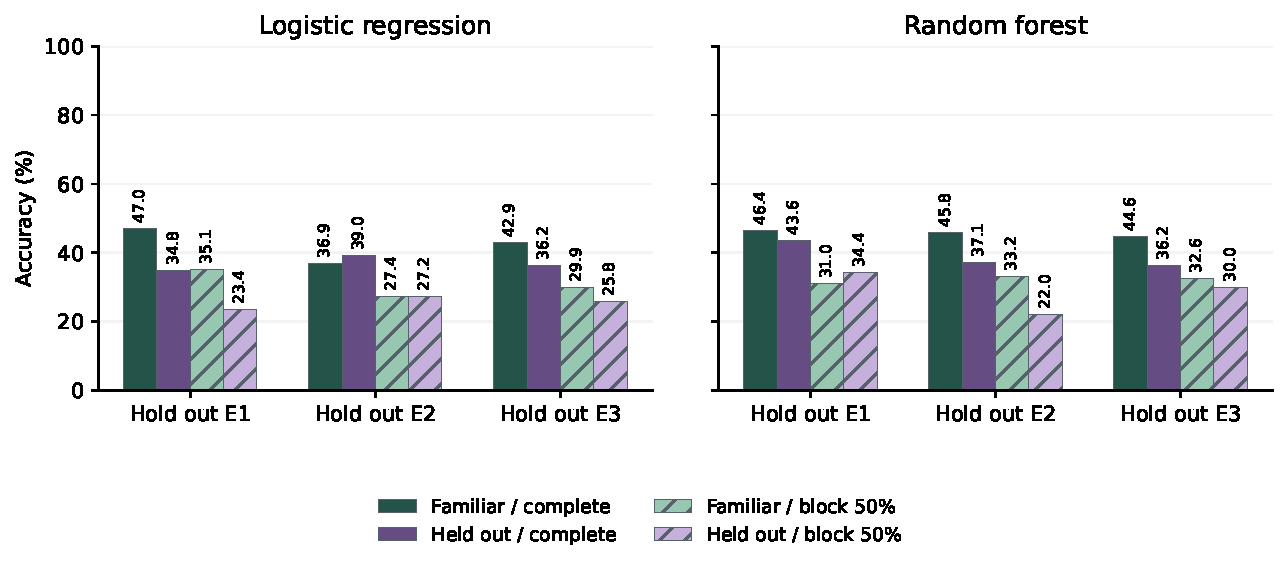
\includegraphics[width=\textwidth]{transfer_accuracy.pdf}
\caption{Classification accuracy on genuine recordings under the declared evaluation. Each group identifies the excluded target environment. Solid bars use complete inputs; hatched bars average five 50\% block-loss masks. Familiar tests exclude training participants, while target tests exclude the whole environment. Counts are 168 familiar and 420 target files per fold. Bars are descriptive; they do not isolate a causal room effect.}
\label{fig:transferaccuracy}
\end{figure*}

Across held-out environments, complete-input accuracy was 462/1,260 (36.7\%) for logistic regression and 491/1,260 (39.0\%) for the forest. At 50\% block loss, the five-mask mean accuracies were 25.5\% and 28.8\%. Random loss at the same fraction gave 31.8\% and 36.6\%. These averages weight the three equally sized target environments equally, and each participant contributes 42 files. They describe fixed lightweight baselines, not the best achievable performance on this dataset.

\begin{center}
\begin{minipage}{\columnwidth}
\refstepcounter{table}\label{tab:transfermetrics}
{\fontsize{9.3}{12}\selectfont\textbf{Table~\thetable.} Pooled held-out metrics. R50/B50 mean random/block loss at 50\%. Accuracy is a percentage; F1 and NLL use native scales.\par}
\vspace{5pt}\begingroup\sffamily\fontsize{9.2}{12}\selectfont
\setlength{\tabcolsep}{5pt}\renewcommand{\arraystretch}{1.45}
\begin{tabularx}{\linewidth}{>{\raggedright\arraybackslash}p{0.31\linewidth}*{3}{>{\centering\arraybackslash}X}}
\rowcolor{indigohead}\multicolumn{1}{l}{\textcolor{white}{\bfseries Condition}} & \multicolumn{1}{c}{\textcolor{white}{\bfseries Acc.}} & \multicolumn{1}{c}{\textcolor{white}{\bfseries Macro F1}} & \multicolumn{1}{c}{\textcolor{white}{\bfseries NLL}}\\
\rowcolor{indigofill}LR clean & 36.7 & 0.363 & 1.659\\
\rowcolor{papergray}LR R50 & 31.8 & 0.330 & 1.780\\
\rowcolor{indigofill}LR B50 & 25.5 & 0.255 & 2.006\\
\rowcolor{papergray}RF clean & 39.0 & 0.392 & 1.443\\
\rowcolor{indigofill}RF R50 & 36.6 & 0.381 & 1.485\\
\rowcolor{papergray}RF B50 & 28.8 & 0.293 & 1.851\\
\end{tabularx}\endgroup
\end{minipage}\end{center}


The probability summaries in Table~\ref{tab:transfermetrics} pool target predictions within each seed, compute the metric, and then average the five corrupted-seed values. In particular, pooled macro F1 is not an average of per-environment F1 scores. Under block loss, NLL increased from 1.659 to 2.006 for logistic regression and from 1.443 to 1.851 for the forest. Multiclass Brier scores increased from 0.764 to 0.889 and from 0.713 to 0.835, respectively. Clean-source calibration therefore did not remove the probability errors associated with corrupted target inputs.

\begin{figure*}[tp]
\centering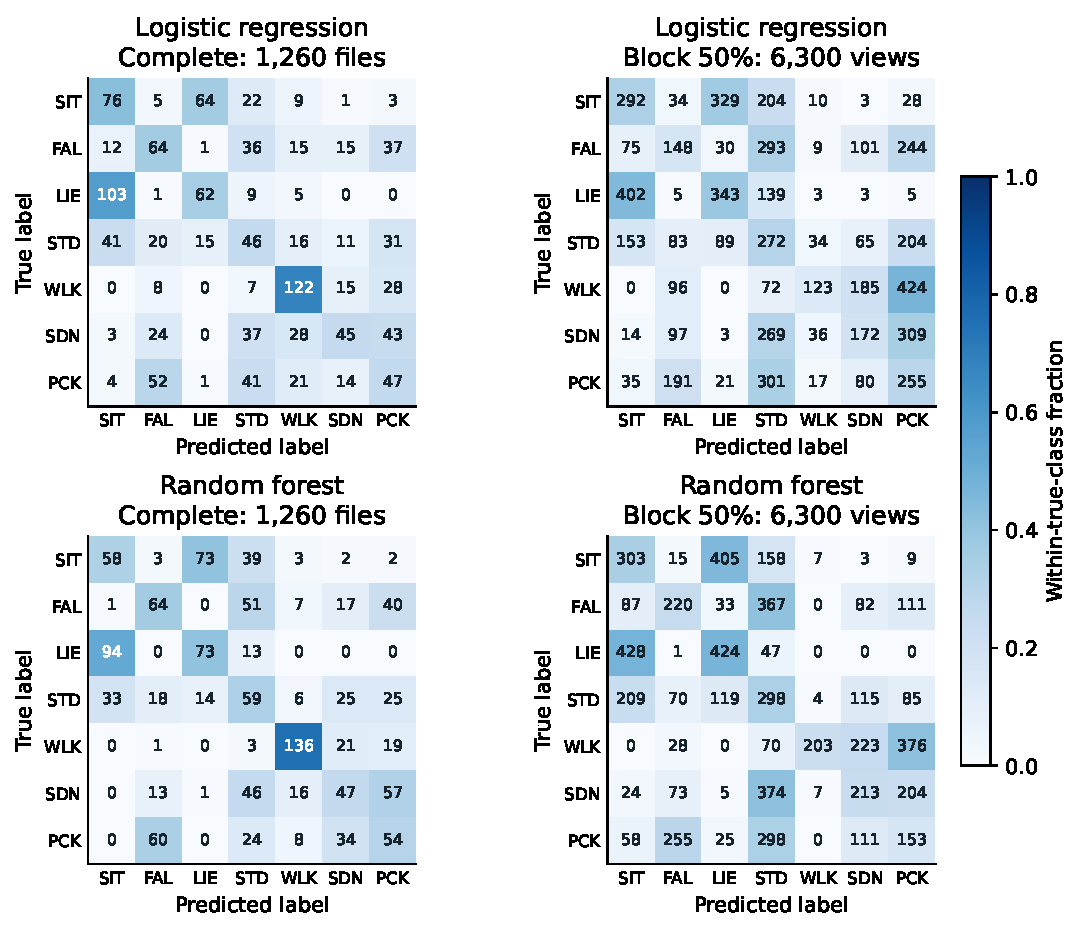
\includegraphics[width=\textwidth]{transfer_confusions.pdf}
\caption{Held-out confusion matrices aggregated across the three fold-specific models of each classifier. Class keys follow Table~\ref{tab:activitymap}. Complete panels contain 1,260 original-file predictions, with 180 files per class. Block panels pool five 50\% masks, giving 6,300 views and 900 per class; these views are dependent repeats. Colors are within-true-class fractions and annotations are counts.}
\label{fig:transferconfusions}
\end{figure*}

Figure~\ref{fig:transferconfusions} shows that aggregate degradation was not uniform across activities. Logistic-regression walking recognition changed from 122/180 complete files to 123/900 masked views; the forest changed from 136/180 to 203/900. Counts in the corrupted panels are repeated views and must not be read as new independent trials. Sitting and lying were frequently confused even on complete inputs, while falls and pen-picking also generated errors. No activity-level safety claim follows from this evaluation.

\section{Interaction contrast and conditional uncertainty}
The sign of $I_q$ in Equation~\ref{eq:interaction} varies with target environment, model, missing fraction, and mask pattern (Figure~\ref{fig:transferinteraction}). For 50\% block loss, LR contrasts were $-0.57$, $+2.29$, and $-2.55$ percentage points for E1--E3. Forest contrasts were $-6.29$, $+2.48$, and $-5.79$ points. Hence the evaluated conditions do not support a uniform superadditive error increase. A negative contrast means the loss-associated error increment was smaller in the target test than in the familiar test; it does not imply robust target performance.

\begin{figure*}[tp]
\centering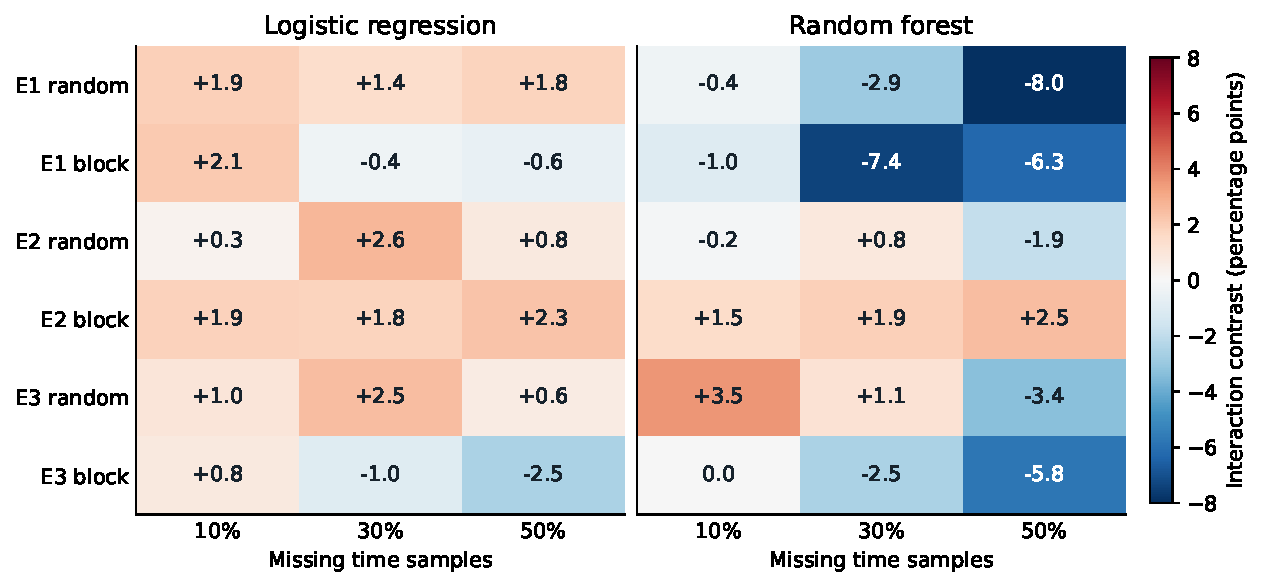
\includegraphics[width=\textwidth]{transfer_interaction.pdf}
\caption{Descriptive difference-in-differences error contrast $100I_q$ in percentage points. Warm colors indicate a larger loss-associated error increase in the held-out domain; cool colors indicate a smaller increase. Zero is the additive reference on this error-rate scale. Each value uses the same clean and masked test files within its domain and averages five masks. Room/cohort confounding and only three environments limit interpretation.}
\label{fig:transferinteraction}
\end{figure*}

For conditional accuracy uncertainty, participant $j$ contributes a mean correctness over its $n_j=42$ files and $S_q$ mask draws:
\begin{equation}
 \begin{aligned}
 a_{j,q}&=\frac{1}{n_jS_q}\sum_{i\in j}\sum_{s=1}^{S_q}
 \mathbb{1}\{\widehat y_{i,q,s}=y_i\},\\
 \widehat A_q&=\frac1{30}\sum_{j=1}^{30}a_{j,q}.
 \end{aligned}
\label{eq:participantaccuracy}
\end{equation}
Here $S_0=1$ for complete inputs and $S_q=5$ for corrupted conditions. A stratified participant bootstrap samples ten IDs with replacement within each of the three target environments, retaining all files and masks of each sampled participant \cite{efron1979}. We use 10,000 draws with a fixed seed and 2.5th--97.5th percentiles (Table~\ref{tab:transferci}).

\begin{center}
\begin{minipage}{\columnwidth}
\refstepcounter{table}\label{tab:transferci}
{\fontsize{9.3}{12}\selectfont\textbf{Table~\thetable.} Conditional participant-resampling ranges for held-out accuracy (\%). They do not cover new environments or model retraining. R50/B50 follow Table~\ref{tab:transfermetrics}.\par}
\vspace{5pt}\begingroup\sffamily\fontsize{9.2}{12}\selectfont
\setlength{\tabcolsep}{5pt}\renewcommand{\arraystretch}{1.45}
\begin{tabularx}{\linewidth}{>{\raggedright\arraybackslash}p{0.31\linewidth}*{2}{>{\centering\arraybackslash}X}}
\rowcolor{plumhead}\multicolumn{1}{l}{\textcolor{white}{\bfseries Condition}} & \multicolumn{1}{c}{\textcolor{white}{\bfseries Accuracy}} & \multicolumn{1}{c}{\textcolor{white}{\bfseries 95\% range}}\\
\rowcolor{plumfill}LR clean & 36.67 & 33.02--40.16\\
\rowcolor{papergray}LR R50 & 31.78 & 28.30--35.22\\
\rowcolor{plumfill}LR B50 & 25.48 & 22.73--28.21\\
\rowcolor{papergray}RF clean & 38.97 & 35.00--42.94\\
\rowcolor{plumfill}RF R50 & 36.60 & 32.46--40.56\\
\rowcolor{papergray}RF B50 & 28.79 & 25.37--32.00\\
\end{tabularx}\endgroup
\end{minipage}\end{center}


The paired clean-to-block accuracy drops were 11.19 percentage points for logistic regression (conditional range 9.16--13.16) and 10.17 for the forest (7.32--12.79). For 50\% random loss, the forest drop was 2.37 points with a range of $-0.40$ to 4.89. Thus this particular random-loss effect is less stable under the declared resampling than its block-loss counterpart.

These ranges preserve the within-person dependence of multiple trials and masks. They assume participant exchangeability within the sampled environments and condition on the already fitted models, selected subset, and mask draws. Training, split-selection, cohort-composition and new-environment uncertainty are excluded. Three environments do not establish a population of deployment sites. We do not attach a significance test or a causal interpretation to the interaction heatmap.

\section{Missingness-informed neural extension}
The extension evaluates four fixed comparators on the same 1,260 files and participant roles: a compact CNN trained on complete source inputs, the same CNN with source-only loss augmentation, MIRA-CSI, and the official basic multivariate MiniRocket transform \cite{dempster2021}. This extension was specified after the classical-baseline audit; it is an additional controlled comparison, rather than a prospectively registered study. It includes five training seeds (20261026--20261030) in each of the three folds, yielding 60 fitted runs. Target labels are used only for scoring.

MIRA-CSI denotes Missingness-Informed Recognition of Activities from Wi-Fi CSI. It adds explicit observation information and coverage-weighted pooling to a temporal CNN. Masks and temporal-gap representations have established precedents, including GRU-D \cite{che2018}; the contribution assessed here is this particular CSI implementation and comparison, not the invention of missingness-aware learning. The amplitude-only clean and augmented CNNs compare training regimes on the same backbone. The initial MIRA-CSI comparison changes mask input, distance input and pooling together and therefore cannot isolate their individual benefits. Section~\ref{sec:components} reports a subsequent component-removal experiment.

Let $B\in\mathbb R^{18\times500}$ denote the amplitude-band representation. Its channel means and standard deviations are estimated only from source-training files. For repaired standardized amplitudes $\widehat B$, the additional gap channel and network input are
\begin{equation}
 d_t=\frac{\min_{s:m_s=1}|t-s|}{500},\qquad
 Z_t=[\widehat B_{:,t};m_t;d_t].
\label{eq:mirainput}
\end{equation}
Distance is measured in normalized packet positions; it is not elapsed time. It is zero at observed positions by construction and can use an observation on either side of a gap. On this integer grid, $m_t=\mathbb I[d_t=0]$, so the distance channel already determines the mask exactly. Removing the explicit mask channel therefore tests an encoding/parameterization choice rather than removing observation-status information. This offline support-distance feature differs from the elapsed-since-previous-observation representation in GRU-D and the retained-sample age relative to a session decision in Zakeri et al. \cite{che2018,zakeri2026age}; it is not a causal streaming feature. Three convolutions use 32, 64 and 128 channels, kernel lengths 7, 5 and 3, stride two, GroupNorm with eight groups, and GELU. If $h_j$ is an encoded temporal feature and $\bar m_j$ the adaptively averaged observation mask at that resolution, pooling is
\begin{equation}
 w_j=\max(\bar m_j,0.05),\qquad
 g=\frac{\sum_jw_jh_j}{\sum_jw_j}.
\label{eq:mirapool}
\end{equation}
The weights describe mask-bin coverage, not calibrated confidence or a physical RF reliability estimate. GroupNorm aggregates statistics across time, so the weights are a coverage heuristic rather than the exact observed fraction of each feature's full dependency set. Dropout (0.2) and a seven-logit linear head complete the network. MIRA-CSI has 40,871 trainable parameters, compared with 40,423 for the amplitude-only CNN. The ordinary CNN uses uniform temporal averaging.

\begin{figure*}[t]
\centering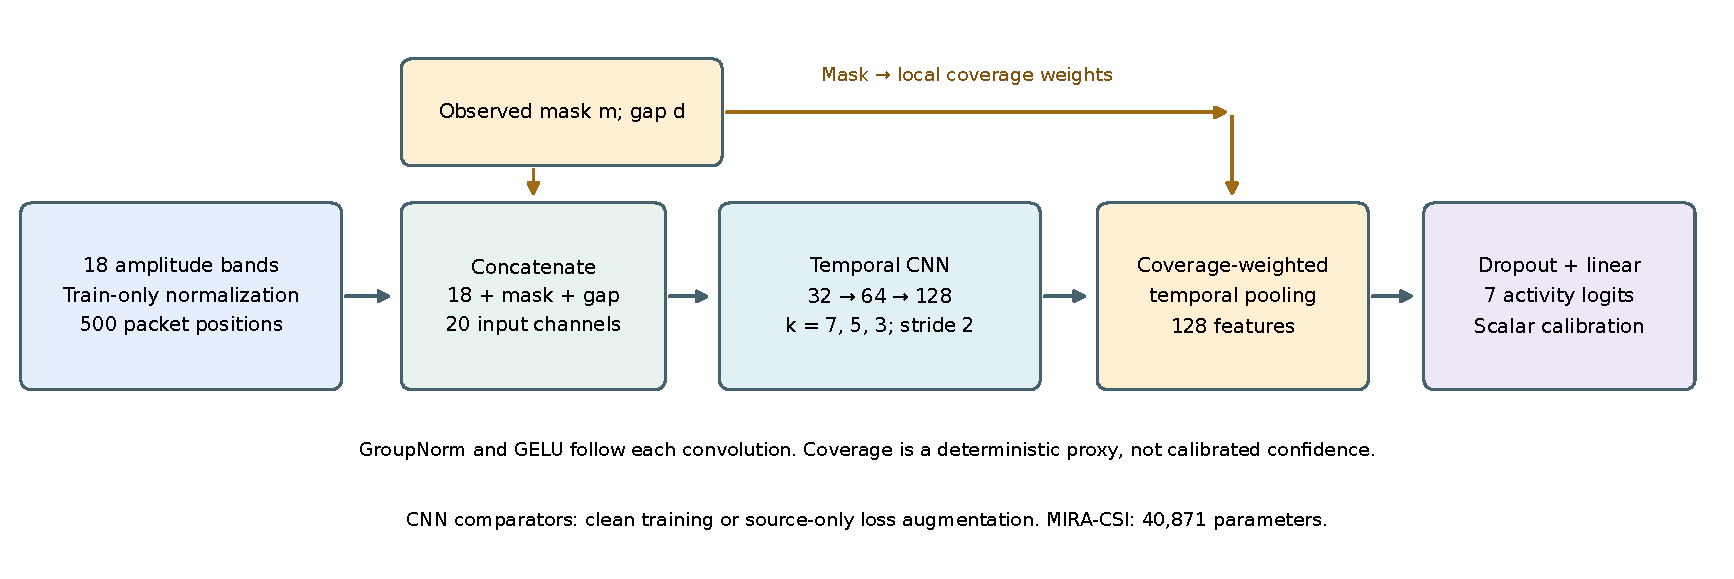
\includegraphics[width=\textwidth]{mira_architecture.pdf}
\caption{Architecture of the implemented MIRA-CSI classifier. Observation mask and distance supplement 18 amplitude bands; mask coverage also weights temporal pooling. The amplitude-only CNN comparators use the same convolutional backbone. These comparators do not isolate the three added components individually. This is an algorithm diagram, not a body reconstruction or a measured RF field.}
\label{fig:miraarchitecture}
\end{figure*}

All CNNs use AdamW (learning rate $10^{-3}$, weight decay $10^{-4}$), batches of 64, at most 60 epochs, and gradient clipping at norm five. Checkpoints minimize clean source-validation cross-entropy, with patience 12 and minimum improvement $10^{-4}$. In both augmented variants each training view remains clean with probability 0.5; otherwise loss pattern, fraction (0.1/0.3/0.5) and repair method are drawn uniformly from their predefined choices. The paired variants use the same independent augmentation-generator draw order for each seed and fold. No target-domain selection is performed. The package retains validation histories and every trained state.

MiniRocket uses the pinned official Numba implementation with 10,000 requested features (9,996 produced), training-only feature scaling without centering, and ridge classification with $\alpha=1$. This compiled comparison is distinct from the earlier 84-feature compatibility check. For every neural or ridge model, a single temperature fitted to clean source-validation logits is frozen on all test conditions.

Three offline repair operators preserve observed values: linear interpolation with held boundaries, nearest observed value (earlier observation on ties), and source-training band mean. These operators do not use hidden values or target labels; interpolation may use later observations and therefore does not establish causal streaming operation. The extended comparison focuses on 50\% random and contiguous loss. A documented compute amendment pairs each training seed with the same mask seed for the primary cross-model comparison, retaining all five fitted seeds and all three folds. The CNNs additionally retain the original five-mask grid as supplementary sensitivity data. Previously completed full-grid MiniRocket output is also retained.

Primary summaries pool the three held-environment prediction sets separately for each seed, then report the mean and sample standard deviation across the five paired training/mask seeds. Familiar summaries pool fold-specific source-test predictions; some familiar files recur across folds and are not independent observations. These standard deviations combine training and mask variation, conditional on the fixed recordings and partitions; they are not population confidence intervals. Repair error is evaluated only at synthetically hidden values using root-mean-square error on the scaled dB amplitude representation.


\section{Extended model and repair results}
The independently checked extension retains all 60 fitted runs, complete probability vectors, validation histories and checkpoints. Table~\ref{tab:expanded} and Figure~\ref{fig:expanded} report the matched primary conditions. Each seed pools three excluded-environment test sets; the five seed summaries describe variation conditional on this selection, rather than five independent datasets.
The compiled MiniRocket reference achieved 53.1\% clean held-environment accuracy and 19.6\% under 50\% block loss with linear repair. MIRA-CSI achieved 23.7\% and 23.0\%, respectively. The CNN comparators and all repair choices are retained; the extension does not impose a target accuracy or establish universal superiority of a model family.

\begin{table*}[t]
\centering\begin{minipage}{\textwidth}
\refstepcounter{table}\label{tab:expanded}
{\fontsize{9.3}{12}\selectfont\textbf{Table~\thetable.} Extended held-environment accuracy (\%). Means $\pm$ sample SD over five paired training/mask seeds; each seed pools 1,260 excluded-environment predictions. R50/B50 denote random/contiguous 50\% loss with linear repair. MR is the compiled 9,996-feature MiniRocket reference.\par}
\vspace{5pt}\begingroup\sffamily\fontsize{9.2}{12}\selectfont
\setlength{\tabcolsep}{5pt}\renewcommand{\arraystretch}{1.45}
\begin{tabularx}{\linewidth}{>{\raggedright\arraybackslash}p{.25\linewidth}*{3}{>{\centering\arraybackslash}X}}
\rowcolor{plumhead}\multicolumn{1}{l}{\textcolor{white}{\bfseries Model}} & \multicolumn{1}{c}{\textcolor{white}{\bfseries Complete}} & \multicolumn{1}{c}{\textcolor{white}{\bfseries R50}} & \multicolumn{1}{c}{\textcolor{white}{\bfseries B50}}\\
\rowcolor{plumfill}CNN & $24.5\pm2.2$ & $24.2\pm2.0$ & $22.2\pm2.1$\\
\rowcolor{papergray}CNN + aug. & $22.5\pm1.8$ & $22.2\pm1.6$ & $20.8\pm1.3$\\
\rowcolor{plumfill}MIRA-CSI & $23.7\pm2.3$ & $22.7\pm2.2$ & $23.0\pm1.3$\\
\rowcolor{papergray}MR (9,996) & $53.1\pm0.3$ & $49.5\pm0.6$ & $19.6\pm0.9$\\
\end{tabularx}\endgroup\end{minipage}\end{table*}

\begin{figure*}[t]
\centering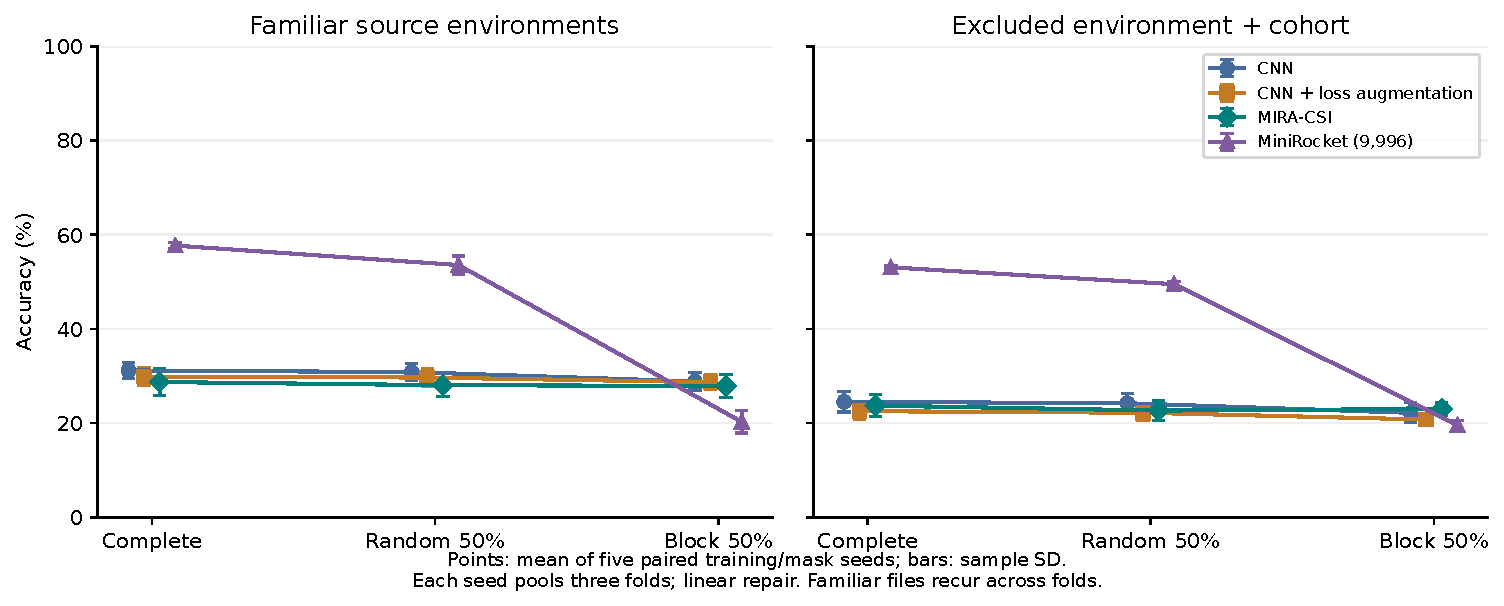
\includegraphics[width=\textwidth]{expanded_comparison.pdf}
\caption{Measured five-seed model comparison. Points are means and bars are sample standard deviations across paired training/mask seeds, with linear repair for corrupted inputs. Held results pool 1,260 distinct files per seed; familiar results pool fold-specific predictions and reuse some files across folds. These bars do not represent uncertainty over new buildings or populations.}
\label{fig:expanded}
\end{figure*}
Relative to the augmented amplitude-only CNN, adding the MIRA inputs and pooling changed pooled held block-loss macro F1 by +0.018 on average (SD 0.023); the paired difference was positive in 5 of five seeds. This is a comparison of the combined modification. It does not isolate mask, distance and pooling effects individually, and it is not a significance test.

\begin{table*}[t]
\centering\begin{minipage}{\textwidth}
\refstepcounter{table}\label{tab:imputers}
{\fontsize{9.3}{12}\selectfont\textbf{Table~\thetable.} Repair and downstream performance at 50\% loss. RMSE is pooled over synthetically hidden amplitude values in scaled dB units. F1 and NLL average five paired seeds after pooling three target folds. MIRA and MR denote MIRA-CSI and MiniRocket (9,996). Repair ground truth is used only for scoring.\par}
\vspace{5pt}\begingroup\sffamily\fontsize{9.0}{12}\selectfont
\setlength{\tabcolsep}{5pt}\renewcommand{\arraystretch}{1.45}
\begin{tabularx}{\linewidth}{>{\raggedright\arraybackslash}p{.12\linewidth}>{\raggedright\arraybackslash}p{.16\linewidth}*{5}{>{\centering\arraybackslash}X}}
\rowcolor{tealhead}\multicolumn{1}{l}{\textcolor{white}{\bfseries Loss}} & \multicolumn{1}{l}{\textcolor{white}{\bfseries Repair}} & \multicolumn{1}{c}{\textcolor{white}{\bfseries RMSE}} & \multicolumn{1}{c}{\textcolor{white}{\bfseries MIRA F1}} & \multicolumn{1}{c}{\textcolor{white}{\bfseries MR F1}} & \multicolumn{1}{c}{\textcolor{white}{\bfseries MIRA NLL}} & \multicolumn{1}{c}{\textcolor{white}{\bfseries MR NLL}}\\
\rowcolor{cyanfill}Random & Linear & 1.03 & 0.209 & 0.487 & 2.140 & 1.593\\
\rowcolor{cyanlight}Random & Nearest & 1.19 & 0.209 & 0.487 & 2.137 & 1.586\\
\rowcolor{cyanfill}Random & Source mean & 3.43 & 0.198 & 0.150 & 2.059 & 3.353\\
\rowcolor{cyanfill}Block & Linear & 2.33 & 0.217 & 0.156 & 2.156 & 5.613\\
\rowcolor{cyanlight}Block & Nearest & 2.58 & 0.216 & 0.180 & 2.137 & 4.517\\
\rowcolor{cyanfill}Block & Source mean & 3.42 & 0.182 & 0.129 & 2.541 & 5.015\\
\end{tabularx}\endgroup\end{minipage}\end{table*}

\begin{figure*}[t]
\centering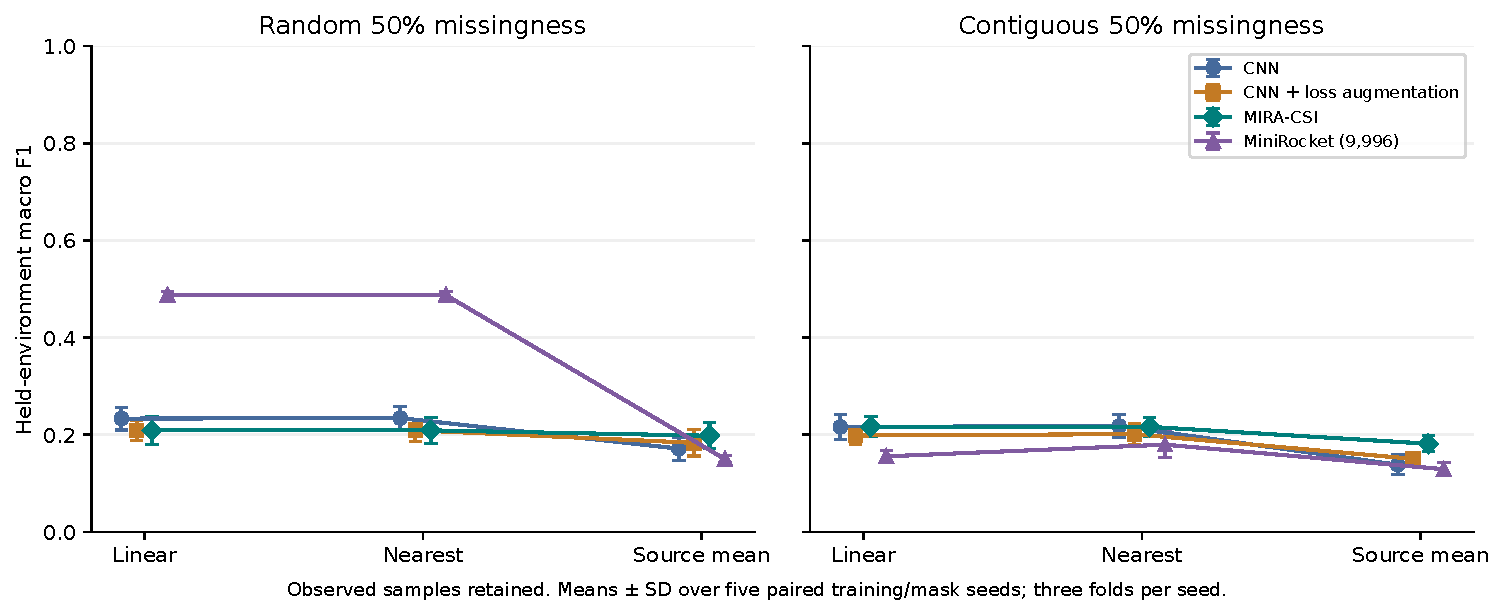
\includegraphics[width=\textwidth]{imputation_comparison.pdf}
\caption{Downstream recognition under three repairs of exactly matched missing positions. Macro F1 pools the three held-environment sets for each seed. Error bars are SD across five paired training/mask seeds. Models and clean-source calibration remain frozen across repair choices; later observations may be used by these offline operators.}
\label{fig:imputation}
\end{figure*}

Table~\ref{tab:imputers} separates signal reconstruction from downstream recognition and probability quality. A lower hidden-value RMSE is not equivalent to a lower classification error: smoothing and class-discriminative variation can respond differently. The saved NLL, Brier and ECE results allow probability quality to be examined without treating a plausible activity label as a calibrated guarantee.

The earlier 84-feature NumPy compatibility check remains in the reproduction archive as a bounded execution audit. It is superseded here by an official compiled transform with 9,996 features and five fitted seeds; its scores and runtime are not pooled with the extension. All new scores are secondary analyses of recorded activities, not demonstrations of live pose reconstruction.


\subsection{Conditional participant-level sensitivity}
A post-hoc analysis of frozen predictions separates the primary five paired-seed summaries from a full mask-grid sensitivity analysis. For each of the three neural configurations, all five training seeds are crossed with all five loss-mask seeds, yielding 25 cells per corrupted condition and five cells for complete inputs. No weights, partitions or temperatures are refitted. Within each cell, predictions from the three held environments are pooled before scoring; the reported estimand averages those cell-level scores, rather than first averaging probability vectors.

For 10,000 bootstrap replicates, ten participant clusters are sampled with replacement independently within each of the three fixed target environments. Each cluster retains its 42 recordings and every saved seed/mask view. Identical resampling weights are applied to all compared models and conditions. The 2.5th and 97.5th percentiles of paired metric differences give the conditional ranges in Table~\ref{tab:conditional}. These ranges condition on the observed rooms, recordings, fitted models, calibration and mask grid; they do not quantify uncertainty over new environments or model retraining. This is an exploratory sensitivity analysis, not a prospectively specified confirmatory test, and its intervals are not adjusted for multiple comparisons.

\begin{table*}[t]
\centering\begin{minipage}{\textwidth}
\refstepcounter{table}\label{tab:conditional}
{\fontsize{9.3}{12}\selectfont\textbf{Table~\thetable.} Full-grid paired differences: MIRA-CSI minus augmented CNN. Each cell shows the point estimate and a conditional 95\% participant-bootstrap percentile range. Accuracy differences are percentage points; macro F1 and NLL differences use their original scales. Positive accuracy/F1 differences and negative NLL differences favour MIRA-CSI. R50/B50 use linear repair.\par}
\vspace{5pt}\begingroup\sffamily\fontsize{9.1}{12}\selectfont
\setlength{\tabcolsep}{5pt}\renewcommand{\arraystretch}{1.55}
\begin{tabularx}{\linewidth}{>{\raggedright\arraybackslash}p{.16\linewidth}*{3}{>{\centering\arraybackslash}X}}
\rowcolor{foresthead}\multicolumn{1}{l}{\textcolor{white}{\bfseries Input}} & \multicolumn{1}{c}{\textcolor{white}{\bfseries $\Delta$ Accuracy (pp)}} & \multicolumn{1}{c}{\textcolor{white}{\bfseries $\Delta$ Macro F1}} & \multicolumn{1}{c}{\textcolor{white}{\bfseries $\Delta$ NLL}}\\
\rowcolor{mintfill}Complete & \shortstack{$+1.19$\\$[-0.14,2.57]$} & \shortstack{$+0.0107$\\$[-0.0043,0.0265]$} & \shortstack{$-0.0354$\\$[-0.0892,0.0174]$}\\
\rowcolor{papergray}R50 & \shortstack{$+0.44$\\$[-1.00,1.88]$} & \shortstack{$+0.0003$\\$[-0.0158,0.0164]$} & \shortstack{$+0.0149$\\$[-0.0358,0.0688]$}\\
\rowcolor{mintfill}B50 & \shortstack{$+1.84$\\$[0.68,3.01]$} & \shortstack{$+0.0136$\\$[0.0005,0.0275]$} & \shortstack{$-0.0410$\\$[-0.0985,0.0158]$}\\
\end{tabularx}\endgroup\end{minipage}\end{table*}

Under contiguous loss, the full-grid macro-F1 difference is smaller than the primary five-pair difference ($0.0136$ versus $0.0182$). The positive conditional classification range is small and unadjusted; the NLL range includes zero. Complete-input and random-loss F1 ranges also include zero. Consequently, this analysis supports at most a narrow, dataset-conditional classification difference under the declared block-loss procedure. It establishes neither general probability-quality improvement nor the separate value of any MIRA-CSI component. Per-environment scores, seed-grid summaries, all declared contrasts, resampling weights and probability-file hashes are retained with this revision.

\section{Component controls and representation sensitivity}\label{sec:components}
\subsection{Frozen component-removal experiment}
A follow-up experiment isolates the explicit mask-input channel, nearest-support-distance input, and coverage-weighted pooling of MIRA-CSI. Four controlled configurations retain the same 20-channel architecture, 40,871 nominal trainable parameters, initialization at each seed, source partitions, augmentation draws, optimizer, checkpoint rule and clean-source temperature calibration. The reference retains all three components. The other configurations respectively zero the mask-input channel, zero the distance-input channel, or replace coverage weighting with uniform temporal averaging. Zeroing an input retains its nominal parameters but removes its data-dependent gradient. In particular, removing the explicit mask input does not remove all missingness information: distance and coverage weighting remain available.

Two standard residual 1D CNNs provide separate architecture-and-capacity comparators, with and without source loss augmentation. Each has three residual blocks of 64/128/128 channels, convolutions of lengths 7/5/3, GroupNorm and GELU, followed by eight-bin temporal averaging and a seven-class head; each has 511,111 parameters. Their architecture is a reference design rather than a new MIRA component. Architecture and parameter count change together, so these models are not component-level ablations and do not isolate a capacity effect. The residual models use the same source-only optimizer, epoch-selection and calibration settings as the compact networks. CUDA-safe explicit temporal-bin means implement the declared pooling operation.

The six configurations, three outer folds and five training seeds produce 90 source-fitted models. All checkpoints and calibration parameters were frozen and hashed before this follow-up evaluation. Each model is tested on complete input and the full five-mask grid of random/contiguous 50\% loss under all three repairs: 31 conditions on both familiar and held sets. This retains 5,580 metric rows and 1,640,520 probability vectors. These are repeated views of the same recordings, not additional participants. Independent arithmetic reconstruction reproduced every metric row, with maximum absolute difference $4.44\times10^{-16}$. A separate CPU audit loaded every frozen checkpoint and reproduced 15,120 source-validation prediction views without a classification-label mismatch; the maximum CPU/T4 logit difference was $6.20\times10^{-6}$.

The follow-up is exploratory: its design responds to results already observed on this dataset. Freezing the new fits prevents target-dependent selection within this execution, but does not make the historical target data an untouched external confirmation set. For a corrupted condition, held predictions are first pooled across the three folds for each training/mask-seed cell. Scores are then averaged across five masks within each training seed, and the mean and sample SD are reported across the five training seeds. This differs from the initial paired-seed summary in Table~\ref{tab:expanded}.

\begin{table*}[t]
\centering\begin{minipage}{\textwidth}
\refstepcounter{table}\label{tab:components}
{\fontsize{9.3}{12}\selectfont\textbf{Table~\thetable.} Frozen follow-up held accuracy (\%). Corrupted conditions average all five mask realizations within each training seed; cells show mean $\pm$ sample SD across five training seeds after pooling the three held sets. R50/B50 use linear repair. All four MIRA configurations have 40,871 nominal trainable parameters; both residual controls have 511,111.\par}
\vspace{5pt}\begingroup\sffamily\fontsize{9.2}{12}\selectfont
\setlength{\tabcolsep}{6pt}\renewcommand{\arraystretch}{1.5}
\begin{tabularx}{\linewidth}{>{\raggedright\arraybackslash}p{.34\linewidth}*{3}{>{\centering\arraybackslash}X}}
\rowcolor{foresthead}\multicolumn{1}{l}{\textcolor{white}{\bfseries Configuration}} & \multicolumn{1}{c}{\textcolor{white}{\bfseries Complete}} & \multicolumn{1}{c}{\textcolor{white}{\bfseries R50}} & \multicolumn{1}{c}{\textcolor{white}{\bfseries B50}}\\
\rowcolor{mintfill}MIRA full reference & $23.73\pm2.26$ & $22.68\pm2.03$ & $22.56\pm1.28$\\
\rowcolor{referencefill}Zero explicit mask input & $23.41\pm1.03$ & $23.22\pm1.23$ & $21.90\pm0.53$\\
\rowcolor{mintfill}Zero distance input & $24.03\pm1.87$ & $22.85\pm1.87$ & $22.77\pm1.02$\\
\rowcolor{referencefill}Uniform temporal pooling & $24.17\pm2.54$ & $23.22\pm1.86$ & $21.30\pm1.57$\\
\rowcolor{lossfill}Residual CNN, clean training & $33.83\pm0.82$ & $33.33\pm0.87$ & $26.72\pm0.67$\\
\rowcolor{shiftfill}Residual CNN, augmented & $30.25\pm1.65$ & $30.09\pm1.70$ & $25.72\pm1.35$\\
\end{tabularx}\endgroup\end{minipage}\end{table*}

\begin{figure*}[t]
\centering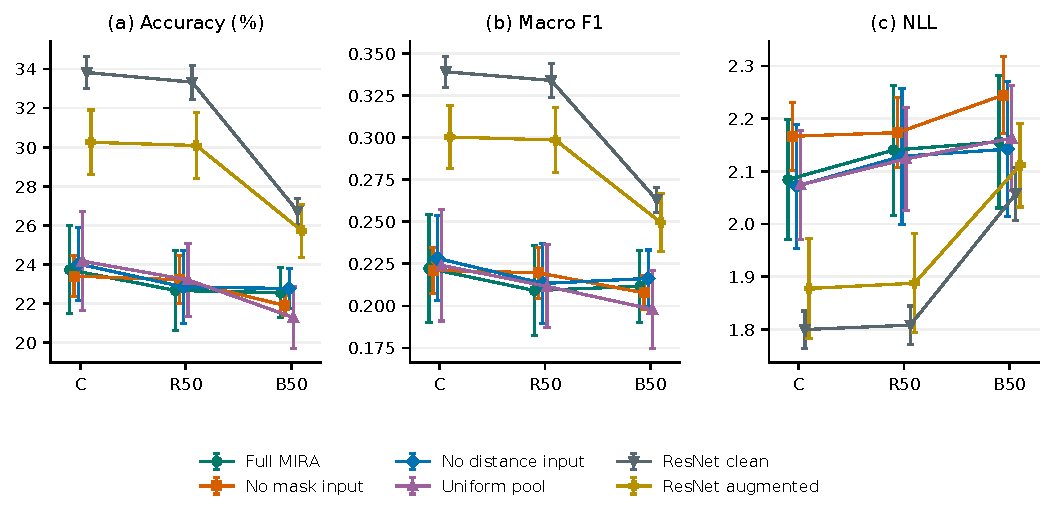
\includegraphics[width=\textwidth]{component_model_comparison.pdf}
\caption{Frozen follow-up comparison of accuracy, macro F1 and source-temperature-calibrated NLL. C is complete input; R50/B50 are random/contiguous 50\% loss with linear repair. Metrics pool 1,260 held files within each training/mask cell, then average masks within training seed. Points show means and bars sample SD across five training seeds on fixed recordings and partitions; they are not confidence intervals for new environments. Higher accuracy/F1 and lower NLL are preferred.}
\label{fig:componentmodels}
\end{figure*}

The larger residual clean-training control reaches 33.83\% held accuracy on complete input and 26.72\% under block loss (Table~\ref{tab:components}, Figure~\ref{fig:componentmodels}); its augmented counterpart reaches 30.25\% and 25.72\%. The residual architectures improve these particular compact-network results, but changing architecture and capacity together does not identify the cause of that difference or establish a generally optimal model. The full MIRA reference reproduces its original clean accuracy. Its block value here averages the full mask grid and therefore differs from the earlier five paired-mask summary. SD across these five mask-averaged seed summaries is not the same quantity as SD across the original five diagonal training/mask pairs. For conditionally independent, identically distributed mask draws within a fixed fit, averaging five masks reduces that fit's mask-variance component by a factor of five; this is not a rule for the total variability across trained models.

For component contrasts, 10,000 paired participant-cluster bootstrap draws sample ten participants with replacement within each fixed environment and retain their complete seed/mask grid. The full model minus each of the three removal controls under linear B50 defines one three-comparison macro-F1 family. Table~\ref{tab:componentcontrasts} reports ordinary 95\% percentile ranges and Bonferroni-adjusted 98.333\% marginal percentile ranges for that family. These approximate conditional sensitivity ranges remain exploratory, depend on within-environment participant exchangeability and fixed fitted models, and do not cover new rooms, retraining or all secondary outcomes. The resampling unit is the participant rather than an individual mask view.

\begin{table*}[t]
\centering\begin{minipage}{\textwidth}
\refstepcounter{table}\label{tab:componentcontrasts}
{\fontsize{9.3}{12}\selectfont\textbf{Table~\thetable.} Component contrasts under contiguous 50\% loss with linear repair. Differences are full MIRA minus the named control in pooled macro F1. The second column adds sample SD of paired, mask-averaged differences across five training seeds; the final column counts positive seed differences. Percentile ranges share identical participant draws, condition on the fixed fitted models, and address only the three contrasts shown.\par}
\vspace{5pt}\begingroup\sffamily\fontsize{9.1}{12}\selectfont
\setlength{\tabcolsep}{5pt}\renewcommand{\arraystretch}{1.5}
\begin{tabularx}{\linewidth}{>{\raggedright\arraybackslash}p{.27\linewidth}>{\centering\arraybackslash}p{.17\linewidth}*{2}{>{\centering\arraybackslash}X}>{\centering\arraybackslash}p{.10\linewidth}}
\rowcolor{purplehead}\multicolumn{1}{l}{\textcolor{white}{\bfseries Control}} & \multicolumn{1}{c}{\textcolor{white}{\bfseries $\Delta$ F1 $\pm$ SD}} & \multicolumn{1}{c}{\textcolor{white}{\bfseries Conditional 95\%}} & \multicolumn{1}{c}{\textcolor{white}{\bfseries Adjusted 98.333\%}} & \multicolumn{1}{c}{\textcolor{white}{\bfseries Positive}}\\
\rowcolor{lavenderfill}Zero explicit mask input & $+0.0039\pm0.0126$ & $[-0.0074,0.0155]$ & $[-0.0096,0.0180]$ & $3/5$\\
\rowcolor{lavenderlight}Zero distance input & $-0.0047\pm0.0117$ & $[-0.0080,-0.0015]$ & $[-0.0086,-0.0007]$ & $2/5$\\
\rowcolor{lavenderfill}Uniform temporal pooling & $+0.0137\pm0.0190$ & $[0.0001,0.0275]$ & $[-0.0023,0.0302]$ & $4/5$\\
\end{tabularx}\endgroup\end{minipage}\end{table*}

The explicit mask-input contrast is inconclusive in this condition. Omitting the distance input gives a small higher mean macro F1 than the full reference, including under the declared conditional three-contrast adjustment; however, the paired difference changes direction across training seeds (Table~\ref{tab:componentcontrasts}). It is not a stable advantage across every initialization. Coverage weighting has a positive unadjusted range, but its adjusted range includes zero (Figure~\ref{fig:componentfamily}). Thus the experiment does not support presenting all three MIRA components as individually beneficial. These condition-specific findings neither prove that a component has no value elsewhere nor validate the full architecture as superior to the reference transform. Different complete-input scores after channel removal are also compatible with retraining under a different parameterization: even a constant clean mask channel can change convolutional activations and the optimization trajectory, including padding-boundary effects. No physical mechanism is identified by that score difference alone.

\begin{figure*}[t]
\centering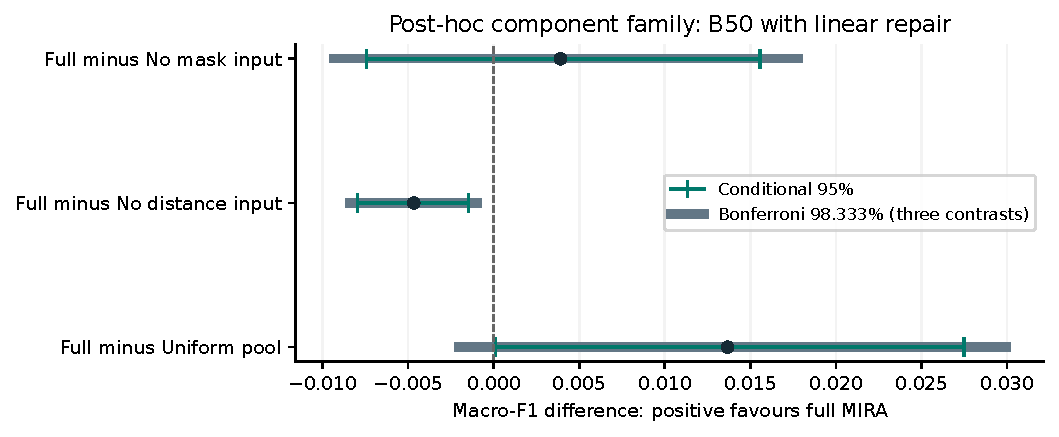
\includegraphics[width=\textwidth]{component_family_intervals.pdf}
\caption{Paired component differences under linear B50. Thin green segments with terminal ticks mark unadjusted 95\% participant-bootstrap percentile ranges; thick gray segments mark 98.333\% ranges adjusted for the three displayed contrasts. Each point is full MIRA minus a removal control, so positive values favour the full model. All ranges use the same 10,000 participant draws within the three fixed environment/cohort strata. This exploratory post-hoc analysis does not measure uncertainty over new environments or model retraining.}
\label{fig:componentfamily}
\end{figure*}


\subsection{Source-selected representation of the reference transform}
A separate clean-input sensitivity study strengthens the known MiniRocket comparator without attributing that algorithm to MIRA-CSI. Before fitting, five candidate input representations were fixed: the original bands, one scalar z-score per recording, a temporal z-score per band, source-training per-band 0.1/99.9-percentile winsorization, and log-mean-power bands. The last candidate averages scaled squared amplitudes before applying $10\log_{10}$ and retains the same 500-position resampling. It uses relative scaled power, not calibrated dBm. Source-only inspection motivated this numerical sensitivity check; changing the transform is not evidence of an architectural contribution.

Within each outer fold, representation selection uses only that fold's source-validation macro F1 at seed 20261026. Validation scores are never pooled across outer folds for selection, because another fold can contain the current target environment. The selected representation is then held fixed across all five seeds. E1 selects per-band temporal standardization; E2 and E3 select scalar recording standardization. MiniRocket remains the official 9,996-feature multivariate transform, with the same source-only feature scaling, ridge coefficient and temperature-fitting rule. All 30 reference/selected fits were sealed before any new held scoring; six seed-one fits were reused and 24 additional fits were trained.

\begin{table*}[t]
\centering\begin{minipage}{\textwidth}
\refstepcounter{table}\label{tab:representation}
{\fontsize{9.3}{12}\selectfont\textbf{Table~\thetable.} Clean-input MiniRocket representation sensitivity. Means $\pm$ sample SD across five seeds; metrics pool 1,260 held files per seed. The selected representation is chosen independently from each outer fold's source validation. This is a reference-transform improvement, not a new MIRA model.\par}
\vspace{5pt}\begingroup\sffamily\fontsize{9.1}{12}\selectfont
\setlength{\tabcolsep}{5pt}\renewcommand{\arraystretch}{1.5}
\begin{tabularx}{\linewidth}{>{\raggedright\arraybackslash}p{.25\linewidth}*{4}{>{\centering\arraybackslash}X}}
\rowcolor{navy}\multicolumn{1}{l}{\textcolor{white}{\bfseries Input representation}} & \multicolumn{1}{c}{\textcolor{white}{\bfseries Accuracy (\%)}} & \multicolumn{1}{c}{\textcolor{white}{\bfseries Macro F1}} & \multicolumn{1}{c}{\textcolor{white}{\bfseries NLL}} & \multicolumn{1}{c}{\textcolor{white}{\bfseries Brier}}\\
\rowcolor{lossfill}Original & $53.08\pm0.33$ & $0.531\pm0.003$ & $1.395\pm0.049$ & $0.639\pm0.008$\\
\rowcolor{shiftfill}Source-selected & $57.44\pm1.04$ & $0.574\pm0.009$ & $1.259\pm0.040$ & $0.586\pm0.013$\\
\end{tabularx}\endgroup\end{minipage}\end{table*}

The pooled accuracy difference is 4.37 percentage points (Table~\ref{tab:representation}). Per-environment mean accuracy changes from 57.24\% to 66.43\% in E1, 50.67\% to 50.43\% in E2, and 51.33\% to 55.48\% in E3. The gain is therefore not shared by every environment. Independent checks reconstructed scores from 12,600 saved held probability vectors and verified all 30 checkpoint hashes without repeating target inference. Recording standardization in this stage uses complete recordings; this clean-only experiment establishes neither missing-input robustness nor an information-safe standardization procedure under hidden-value loss. No inference about a new MIRA mechanism follows from the MiniRocket improvement.

The selected pipeline's seed SD is 1.04 percentage points, compared with 0.33 for the original representation. The representation choice is fixed from one source-validation seed; its stability across alternative selection seeds has not been measured. Furthermore, the CNNs were not subjected to the same five-candidate input-selection procedure. This sensitivity result therefore compares two declared MiniRocket pipelines and does not isolate an architectural cause for their differences from the neural models.


\section{Probability quality and selective ranking}
A descriptive post-hoc audit examines the already frozen neural and ridge predictions without fitting another model, temperature or threshold. Table~\ref{tab:properquality} and Figure~\ref{fig:neuralrisk} retain the initial 60-fit package with five paired training/mask seeds; they are not the full-grid follow-up. Figure~\ref{fig:componentmodels} and the follow-up score files report the 90-fit comparison, including both residual controls, using mask-averaged seed summaries. Table~\ref{tab:properquality} reports proper scores alongside macro F1 and ECE. Because every pooled held set is balanced over seven classes, the uninformative reference distribution $p_k=1/7$ has
\begin{equation}
 \mathrm{NLL}_{\rm unif}=\log 7\approx1.946,\qquad
 \mathrm{Brier}_{\rm unif}=1-\frac17\approx0.857.
\label{eq:uniformreference}
\end{equation}
This is a proper-score comparison, not a claim that uniform probabilities identify activities. Tied uniform confidence also cannot define a meaningful rejection ranking without an additional rule.

The mean NLL and Brier values for all three compact neural configurations exceed this uninformative reference on both complete and block-masked target inputs. Their accuracy above the balanced-class chance level therefore does not establish useful probabilistic confidence. MiniRocket improves both proper scores on complete inputs, but its block-loss NLL and Brier are markedly worse. Clean-source temperature scaling does not transfer a calibration guarantee to the excluded environment and cohort.

\begin{table*}[t]
\centering\begin{minipage}{\textwidth}
\refstepcounter{table}\label{tab:properquality}
{\fontsize{9.3}{12}\selectfont\textbf{Table~\thetable.} Held-environment probability quality and macro F1. C: complete input; B50: contiguous 50\% loss with linear repair. Values are means $\pm$ sample SD over five paired seeds after pooling three folds. NLL, summed multiclass Brier and ECE are lower-is-better; F1 is higher-is-better. The uniform distribution is an untrained proper-score reference, not a useful activity discriminator.\par}
\vspace{5pt}\begingroup\sffamily\fontsize{9.0}{12}\selectfont
\setlength{\tabcolsep}{5pt}\renewcommand{\arraystretch}{1.45}
\begin{tabularx}{\linewidth}{>{\raggedright\arraybackslash}p{.19\linewidth}>{\centering\arraybackslash}p{.065\linewidth}*{4}{>{\centering\arraybackslash}X}}
\rowcolor{indigohead}\multicolumn{1}{l}{\textcolor{white}{\bfseries Model}} & \multicolumn{1}{c}{\textcolor{white}{\bfseries Input}} & \multicolumn{1}{c}{\textcolor{white}{\bfseries NLL}} & \multicolumn{1}{c}{\textcolor{white}{\bfseries Brier}} & \multicolumn{1}{c}{\textcolor{white}{\bfseries ECE}} & \multicolumn{1}{c}{\textcolor{white}{\bfseries Macro F1}}\\
\rowcolor{indigofill}CNN & C & $2.091\pm0.053$ & $0.915\pm0.020$ & $0.197\pm0.026$ & $0.235\pm0.025$\\
\rowcolor{indigofill}CNN & B50 & $2.183\pm0.046$ & $0.941\pm0.017$ & $0.227\pm0.026$ & $0.216\pm0.026$\\
\rowcolor{papergray}CNN + aug. & C & $2.120\pm0.059$ & $0.928\pm0.022$ & $0.205\pm0.032$ & $0.212\pm0.023$\\
\rowcolor{papergray}CNN + aug. & B50 & $2.199\pm0.052$ & $0.951\pm0.018$ & $0.230\pm0.024$ & $0.199\pm0.019$\\
\rowcolor{indigofill}MIRA-CSI & C & $2.084\pm0.114$ & $0.908\pm0.030$ & $0.184\pm0.041$ & $0.222\pm0.032$\\
\rowcolor{indigofill}MIRA-CSI & B50 & $2.156\pm0.130$ & $0.927\pm0.031$ & $0.207\pm0.042$ & $0.217\pm0.021$\\
\rowcolor{papergray}MR (9,996) & C & $1.395\pm0.049$ & $0.639\pm0.008$ & $0.124\pm0.009$ & $0.531\pm0.003$\\
\rowcolor{papergray}MR (9,996) & B50 & $5.613\pm0.430$ & $1.370\pm0.037$ & $0.633\pm0.028$ & $0.156\pm0.012$\\
\rowcolor{jointfill}Uniform reference & -- & 1.946 & 0.857 & -- & --\\
\end{tabularx}\endgroup\end{minipage}\end{table*}

\begin{figure*}[t]
\centering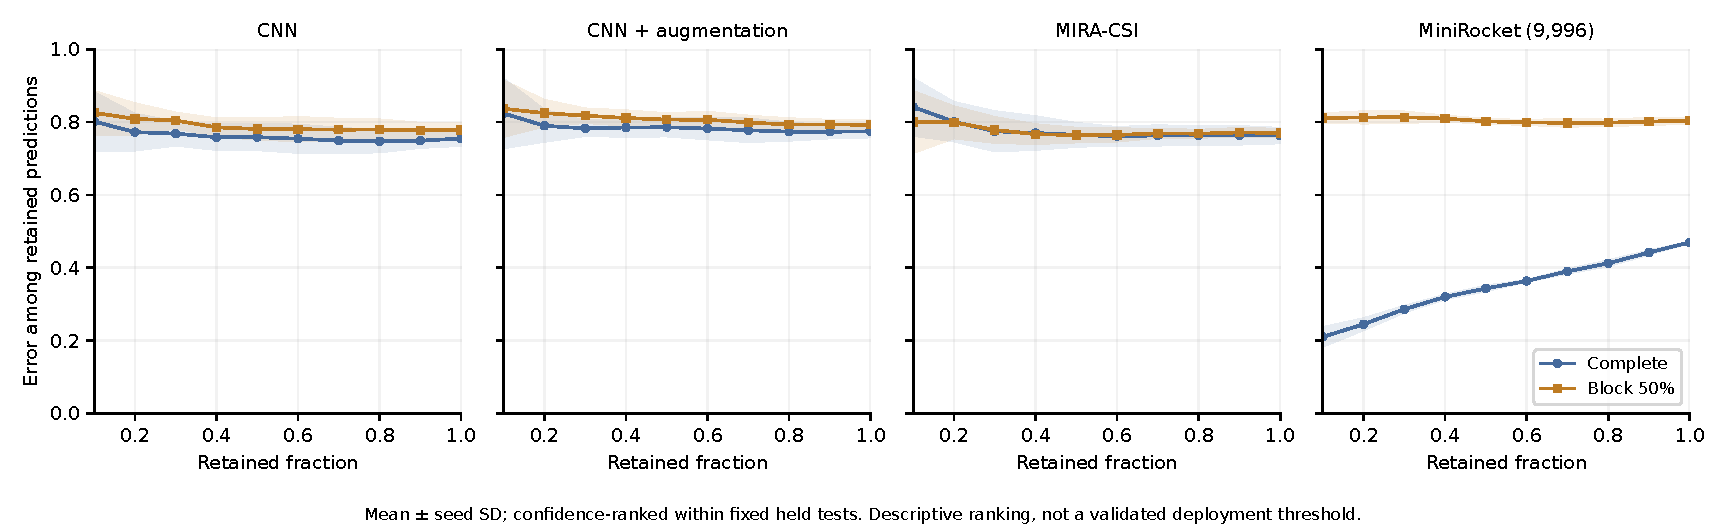
\includegraphics[width=\textwidth]{neural_risk_coverage.pdf}
\caption{Descriptive risk--coverage curves of frozen models on held environments. At each retained fraction, predictions are ranked by maximum calibrated probability within that test condition. Lines average five paired seeds; shading is sample SD, not a population confidence interval. Confidence ranking selects observations; labels are used only to calculate retained error. The curves do not validate a deployable threshold.}
\label{fig:neuralrisk}
\end{figure*}

At 80\% retained coverage under block loss, mean selective error was 76.8\% for MIRA-CSI and 79.8\% for MiniRocket. Thus, retaining high-confidence predictions is not sufficient to guarantee low error in these target conditions. Figure~\ref{fig:neuralrisk} records the complete coverage range rather than choosing a favorable operating point. These are conditional error descriptions, not a validated selective-risk bound.

\section{Exploratory support-matched spectral extension}
\label{sec:m2-extension}

The earlier results motivate a separate investigation of the representation and
fusion used by MIRA-CSI, rather than an assumption that a larger neural model
must improve transfer. We evaluate five explicitly defined arms, A--E, in a
frozen 75-fit execution. The research direction was developed after historical
target outcomes had been observed. Although all five arms and the primary
comparison were fixed before this execution's test evaluation, the extension
is exploratory, not a fresh preregistered confirmation. E was a declared
feature-only comparator; its prominence below follows its observed result and
must not be retrospectively presented as the original main hypothesis.

\subsection*{Prior work and scope of the construction}
Covariance-based CSI features predate this extension. PADS uses eigenvalues of
covariance matrices from normalized CSI amplitude and phase for binary motion
detection~\cite{m2pads}. Covariance-normalized temporal variation also has a
long history: slow feature analysis (SFA) minimizes temporal change under
variance/decorrelation constraints~\cite{m2sfa}, while second-order blind
identification (SOBI) uses joint diagonalization of lagged covariance matrices
for source separation~\cite{m2sobi}. The present classifier is neither a new
invention of covariance eigenspectra nor an implementation of SFA or SOBI.
It combines an explicitly defined observed-endpoint normalization with a
fixed cell/lag grid and compares its use in feature-only and hybrid models.
PADS's binary task and acquisition protocol are not a matched seven-class
baseline, so its reported detection rates are not compared with our accuracy.

Missingness indicators and elapsed-time information are established model
inputs~\cite{che2018}. Mask-aware renormalized filtering likewise has prior
art~\cite{m2partial}; the CNN here does not implement the partial-convolution
mask-update rule. Our distance is the normalized distance to the nearest
observed position in either direction, making the implementation offline.
We claim neither causal streaming nor a new principle of missing-data handling.

\subsection*{Data representation and source-only roles}
We retain the existing immutable selection of 1,260 genuine recordings from
the public Alsaify et al. dataset~\cite{multienvdata}: 30 participants, ten in each
of three environments, seven selected activity segments and six selected
trials per subject/segment. This subset is not the entire source dataset.
The seven labels are sitting, falling from sitting, lying, standing, walking
between transmitter and receiver, sitting down, and picking up an object.

This extension uses a fixed \emph{log-mean scaled power} representation, which
differs from the earlier mean-log-amplitude representation. Let
$H^{\mathrm{sc}}_{r,k}(j)$ be the previously scaled complex CSI for receive
antenna $r$, exported-subcarrier index $k$ and valid packet index $j$.
For consecutive groups $\mathcal G_b$ of five exported subcarriers, the fixed
per-record conversion is
\begin{equation}
 q_{r,b}(j)=10\log_{10}\!\left[
 \max\!\left\{\frac{1}{5}\sum_{k\in\mathcal G_b}
 |H^{\mathrm{sc}}_{r,k}(j)|^2,10^{-24}\right\}\right].
 \label{eq:m2-power}
\end{equation}
Three receiving antennas and six groups yield 18 streams, each linearly
resampled to 500 equally spaced valid-packet-index positions. These are dB
values of dimensionless scaled channel power, not calibrated dBm, body heat,
or a physical image. Original recording duration and irregular packet timing
are not preserved. The conversion is recordwise and unfitted; no pooled target
statistics are used. Changing this representation is a preprocessing choice,
not evidence of a new sensing capability.

For each excluded environment $e\in\{1,2,3\}$, the other two environments
provide 504 source-training recordings from 12 participants, 168 validation
recordings from four other participants, and 168 familiar-environment test
recordings from another four participants. All 420 recordings from the ten
participants in $e$ form the held-environment test. Participants are disjoint
between roles within each fold. Since each environment has a different
participant cohort, this evaluates joint environment--cohort transfer; it
cannot identify a causal room effect. Familiar-test participants can recur in
other outer folds, so familiar scores are reported per fold, not treated as
independent new cohorts in a pooled confidence calculation.

Per-band population means and standard deviations are fitted only over source
training files and positions. Standard deviations have a $10^{-6}$ lower
bound. The temporal path subtracts/divides those statistics only at observed
entries, then assigns exact zero to hidden entries. The fixed spectral branch
uses the raw observed values of the processed power tensor. Consequently its
no-hidden-value property concerns simulated loss \emph{after} the fixed
packet-index conversion, not missing raw acquisition packets before
resampling or power scaling.

\subsection*{Matched endpoint statistics and numerical implementation}
Write $x_t\in\mathbb R^{18}$ for one processed recording and
$m_t\in\{0,1\}$ for its shared temporal observation mask. For a cell
$B=[a,b)$ and lag $\ell$, retain the original index pairs
\begin{equation}
 \begin{aligned}
 \mathcal P_{B,\ell}&=
 \{t:a\leq t<b-\ell,\ m_t=m_{t+\ell}=1\},\\
 n&=|\mathcal P_{B,\ell}|.
 \end{aligned}
 \label{eq:m2-pairs}
\end{equation}
Only the two endpoints need be observed. Missing interior positions do not
remove a pair, and remaining observations are never compressed together.
For $a_i=x_{t_i}$ and $b_i=x_{t_i+\ell}$, define
\begin{align}
 \mu_P&=\frac{1}{2n}\sum_{i=1}^{n}(a_i+b_i),\label{eq:m2-mean}\\
 N&=\frac{1}{2n}\sum_{i=1}^{n}(b_i-a_i)(b_i-a_i)^\top,\label{eq:m2-N}\\
 D_P&=\frac{1}{2n}\sum_{i=1}^{n}
 \big[(a_i-\mu_P)(a_i-\mu_P)^\top\nonumber\\[-2pt]
 &\hspace{28mm}+(b_i-\mu_P)(b_i-\mu_P)^\top\big].\label{eq:m2-D}
\end{align}
Here $N$ is an \emph{uncentered increment second moment}, with the intentional
factor $1/2$; it is not the covariance of mean-subtracted increments. Both
moments use the same multiset of observed pair endpoints. A position can
occur in more than one pair, so endpoint multiplicities enter $D_P$.

With $u_i=a_i-\mu_P$ and $v_i=b_i-\mu_P$,
\begin{equation}
 2D_P-N=\frac{1}{2n}\sum_i(u_i+v_i)(u_i+v_i)^\top\succeq0.
 \label{eq:m2-bound}
\end{equation}
Thus $0\preceq N\preceq2D_P$. Since
$\ker(D_P)\subseteq\ker(N)$, the finite generalized spectrum on the full
effective covariance support lies in $[0,2]$. This algebraic property defines
the construction; it is not an empirical guarantee of correct classification.

The implementation computes symmetric float64 moments and diagonalizes $D_P$.
If $D_P=U\operatorname{diag}(d_i)U^\top$, retain
$I=\{i:d_i>10^{-8}d_{\max}\}$. It forms
\begin{equation}
 W=\operatorname{diag}(d_i^{-1/2})_{i\in I}U_I^\top,\qquad
 \lambda=\operatorname{eig}(WNW^\top).
 \label{eq:m2-whiten}
\end{equation}
The matrix is symmetrized before eigendecomposition. A violations tolerance
of $10^{-4}$ is used: violations beyond the allowed negative or matched upper
bound raise an error, while small allowed violations are clipped. The retained
eigenvalues are sorted and transformed as
\begin{equation}
 z_i=\log\big(0.999\lambda_i+0.001\big).
 \label{eq:m2-log}
\end{equation}
Eighteen entries are reserved per cell/lag; unused entries are zero, equivalent
to the neutral transformed value at $\lambda=1$. With fewer than 36 endpoint
pairs or zero effective rank, the block is neutral and its validity flag is
zero. No difficult recording is dropped. A valid block's flag is one; the
pair fraction $n/(b-a-\ell)$ is also retained. Padding does not uniquely
identify rank, and neither flag nor pair fraction is a physical confidence.

The cells are $[0,500)$, $[0,250)$ and $[250,500)$, with lags
$\{1,2,4,8,16,32\}$. Across 18 cell/lag combinations, concatenating
$18\times18=324$ spectral entries, 18 validity flags and 18 pair fractions
gives 360 float32 classifier inputs. Fully observed per-record features are
cached; a corrupted recording's features are recomputed under its actual mask.
No clean hidden values are supplied through the cache.

For the all-observed comparator B, $N$ is unchanged but $D_P$ is replaced by
\begin{equation}
 \begin{aligned}
 D_O&=\frac{1}{M}\sum_{t\in O_B}(x_t-\mu_O)(x_t-\mu_O)^\top,\\
 O_B&=\{t\in B:m_t=1\}.
 \end{aligned}
 \label{eq:m2-B}
\end{equation}
Here $M=|O_B|$ and $\mu_O$ is the uniform observed-cell mean. B's spectrum
need not be bounded above by 2 and is not clipped at 2. This comparator
changes endpoint weighting, centering, and potentially included positions.
It differs from A even when every position is observed: for non-cyclic lag-1
pairs, endpoint multiplicities are $[1,2,\ldots,2,1]$ rather than uniform.
Therefore A--B does not isolate an effect present only under missingness.

C replaces the full-matrix quotients by matched per-channel diagonal ratios
$N_{jj}/(D_P)_{jj}$ in fixed channel order. Positive diagonal variance is
required; zero-variance channels receive neutral ratio 1, and an entirely
zero-variance block is invalid. Unlike A/B, C has no relative full-matrix
rank threshold or sorted-spectrum padding. It is a useful simpler alternative,
not a pure deletion of off-diagonal entries with every other rule unchanged.

\paragraph{Scope of invariance.}
For the same mask, cell and lag, an ideal fixed nonsingular affine channel
map $x'_t=Gx_t+c$ yields $N'=GNG^\top$ and $D'_P=GD_PG^\top$.
The untruncated generalized spectrum on the full effective support is
unchanged. \emph{B shares this ideal congruence invariance}, because its
observed-cell covariance obeys the same transformation law. Matching supplies
the common endpoint reference and the $[0,2]$ bound, not the origin of
invariance absent from B. This nuisance model is not a physical law for
arbitrary room, participant, multipath or antenna changes.

The implemented threshold can change the retained subspace even if the
retained rank does not change. For example, use three active directions with
$D=\operatorname{diag}(1,9\times10^{-9},2\times10^{-8})$ and
$N=D\operatorname{diag}(0.2,0.8,1.5)$. Under
$G=\operatorname{diag}(1,2,0.5)$, whose condition number is 4, the relative
threshold retains rank 2 before and after transformation, but the retained
spectra change from $[0.2,1.5]$ to $[0.2,0.8]$. Exact null directions can pad
this example to 18 dimensions. Stable retained subspaces and adequate numerical
conditioning, not merely unchanged rank, are required for a numerical
invariance approximation. The threshold, clipping, log floor and padding
qualify the implementation; the hybrid CNN is not generally affine invariant.

\subsection*{Arms, training and frozen evaluation}
Table~\ref{tab:m2-arms} defines all five arms. For A--D, the temporal encoder
receives 18 normalized channels, the mask, and the symmetric nearest-observation
distance divided by 500. Three Conv1d blocks use output widths 32, 64, 128;
kernels 7, 5, 3; stride 2 and same-style padding; each is followed by
eight-group GroupNorm and GELU. Final temporal pooling weights are adaptive
averages of the mask, lower bounded by 0.05. GroupNorm mixes temporal positions;
these weights are a heuristic, not exact local receptive-field support.

For A--C and E, a 360--64--32 MLP with GELU after each linear layer encodes
the fixed features. A--C concatenate this vector with the 128-dimensional
temporal representation; D retains only the temporal vector; E retains only
the feature vector. Dropout 0.2 precedes a seven-logit linear classifier.
The trainable counts are 66,279 for A/B/C, 40,871 for D and 25,415 for E.
Removing a path also changes capacity, so D/E are not parameter-matched
interventions that identify a unique cause.

All arms use the settings in Table~\ref{tab:m2-protocol}: AdamW with learning
rate $10^{-3}$ and weight decay $10^{-4}$, cross-entropy, batch size 64,
gradient-norm clipping at 5, at most 60 epochs, and stopping after 12 epochs
without a clean source-validation NLL decrease exceeding $10^{-4}$.
The saved best validation-NLL weights are restored. One scalar temperature
$T\in[0.1,10]$ is then fitted on that same clean source validation set by
bounded NLL minimization, following the established temperature-scaling
approach~\cite{guo2017}. Neither fitting step uses familiar or held
recordings to fit or select parameters. The weights and temperature are fixed for all test conditions;
source-only calibration does not guarantee calibration after transfer.

Training retains complete input with probability 0.5. Otherwise it draws
random or contiguous loss uniformly and a missing fraction from
$\{0.1,0.3,0.5\}$ uniformly. Masks are shared across channels and independent
of class labels. A separate NumPy generator resets per training seed, so the
source permutation and augmentation draws match across arms irrespective of
Torch/dropout random-number consumption. There is no choice among imputers:
the implementation uses observed entries with canonical zero-fill and actual-
mask features. Repeating multiple hidden fills would duplicate the same
defined input path rather than measure different repairs.

Training seeds are 20261026--20261030. Five arms, three outer folds and five
seeds give 75 source fits. All final checkpoints, source calibration values,
validation outputs and implementation/input hashes were frozen together and
independently audited before held/familiar model inference. Static per-record
preprocessing and hash reads are distinct from inference or target fitting.
An explicit evaluation-only stage then tested complete input, random 50\%
loss under five fixed mask seeds, and contiguous 50\% loss under the same
five seeds: 11 conditions per fit. Each loss mask removes exactly 250 of the
500 normalized positions, shared across all 18 channels. These are synthetic
post-conversion deletions, not measured wireless outages.

\begin{table*}[t]
\centering
\caption{Frozen comparison arms. All arms use the same source partitions, augmentation draw sequence and optimization settings. A--C have identical nominal trainable parameter counts; D and E change capacity as well as their input paths. The table defines controls, not claims of isolated causal mechanisms.}
\label{tab:m2-arms}
\begingroup\fontsize{9.5}{12}\selectfont
\setlength{\tabcolsep}{5pt}\renewcommand{\arraystretch}{1.13}
\setlength{\extrarowheight}{1.3pt}\setlength{\arrayrulewidth}{0.5pt}\arrayrulecolor{m2border}
\begin{tabularx}{\textwidth}{|llr>{\raggedright\arraybackslash}X|}
\hline\rowcolor{m2head}
\mTwoHead{Arm} & \mTwoHead{Paths} & \mTwoHead{Parameters} & \mTwoHead{Fixed-feature construction} \\
\hline
\rowcolor{m2Afill} A & Temporal + feature MLP & 66,279 & Matched-endpoint generalized lagged-increment spectrum. \\
\hline
\rowcolor{m2Bfill} B & Temporal + feature MLP & 66,279 & Same increment numerator; covariance denominator over all observed cell positions. \\
\hline
\rowcolor{m2Cfill} C & Temporal + feature MLP & 66,279 & Matched per-channel diagonal ratios, kept in channel order. \\
\hline
\rowcolor{m2Dfill} D & Temporal only & 40,871 & No fixed spectral or ratio feature branch. \\
\hline
\rowcolor{m2Efill} E & Feature MLP only & 25,415 & Exactly A's fixed features, without the temporal CNN. \\
\hline
\end{tabularx}
\arrayrulecolor{black}\endgroup
\end{table*}

\begin{table*}[t]
\centering
\caption{Executed extension protocol. This is an exploratory follow-up with historical target outcomes already known; freezing this execution does not make the research direction a fresh preregistered hypothesis.}
\label{tab:m2-protocol}
\begingroup\fontsize{9.5}{12}\selectfont
\setlength{\tabcolsep}{5pt}\renewcommand{\arraystretch}{1.13}
\setlength{\extrarowheight}{1.3pt}\setlength{\arrayrulewidth}{0.5pt}\arrayrulecolor{m2border}
\begin{tabularx}{\textwidth}{|>{\raggedright\arraybackslash}p{.22\textwidth}>{\raggedright\arraybackslash}X|}
\hline\rowcolor{m2head}
\mTwoHead{Item} & \mTwoHead{Executed setting} \\
\hline
\rowcolor{m2Afill} Input & 1,260 selected real recordings; 18 fixed log-mean-power streams by 500 normalized packet positions. \\
\hline
\rowcolor{m2Bfill} Outer-fold roles & 504 training, 168 validation, 168 familiar-test, 420 held-environment recordings. Participants are disjoint within each fold. \\
\hline
\rowcolor{m2Afill} Fixed feature grid & Whole record and two half-record cells; lags 1, 2, 4, 8, 16, 32; at least 36 observed endpoint pairs; 360 features. \\
\hline
\rowcolor{m2Bfill} Numerical choices & Relative covariance eigenvalue threshold $10^{-8}$; log mixture $10^{-3}$; bound violation tolerance $10^{-4}$. \\
\hline
\rowcolor{m2Afill} Training & AdamW, learning rate $10^{-3}$, weight decay $10^{-4}$, batch 64, gradient-norm clip 5, dropout 0.2, at most 60 epochs. \\
\hline
\rowcolor{m2Bfill} Stopping and calibration & Clean source-validation NLL, minimum decrease $10^{-4}$, patience 12; one validation temperature in $[0.1,10]$. \\
\hline
\rowcolor{m2Afill} Augmentation & Probability 0.5 complete; otherwise uniform random/contiguous loss and uniform fraction 0.1/0.3/0.5, same record order and draw sequence for all arms. \\
\hline
\rowcolor{m2Bfill} Repetitions & Training seeds 20261026--20261030; five arms by three folds by five seeds = 75 fits. Five fixed test masks per loss pattern. \\
\hline
\rowcolor{m2Afill} Evaluation & Complete, random 50\%, contiguous 50\%; 11 realizations per fit; all 75 weights and calibration values frozen before held/familiar inference. \\
\hline
\rowcolor{m2Bfill} Primary comparison & A minus B pooled held macro F1 under contiguous 50\% loss. Other arms, input conditions and metrics remain visible. \\
\hline
\end{tabularx}
\arrayrulecolor{black}\endgroup
\end{table*}


The primary contrast remains A minus B held macro F1 under contiguous
50\% loss. For each training-seed/mask-seed cell, we first concatenate the
three disjoint held-fold predictions and score the resulting 1,260 recordings.
For a metric $g$, with $S=5$ training seeds and $K=5$ masks under loss,
\begin{equation}
 \begin{aligned}
 \bar g_s&=\frac1K\sum_{k=1}^{K}g_{s,k},\qquad
 \bar g=\frac1S\sum_{s=1}^{S}\bar g_s,\\
 s_g^2&=\frac1{S-1}\sum_s(\bar g_s-\bar g)^2.
 \end{aligned}
 \label{eq:m2-summary}
\end{equation}
Complete input uses $K=1$. Macro F1 is recomputed from each concatenated
seven-class confusion matrix, rather than averaging fold F1 values.
Per-fold held and familiar metrics are summarized separately by the same
mask-first/seed-second rule. Reported SD is variation over five training seeds
on fixed data, not a participant-population confidence interval. Repeated
masks and fold reuse do not create new independent participants.

For probabilities $p_{ic}$ and class labels $y_i$, NLL is
$-n^{-1}\sum_i\log p_{i,y_i}$ using stable source-temperature log-softmax.
The multiclass Brier score is
$n^{-1}\sum_i\sum_{c=1}^{7}(p_{ic}-\mathbf1[y_i=c])^2$; it is summed over
classes, not divided by seven. Accuracy and unweighted seven-class macro F1
are also retained. Independent audit recomputed metrics directly from saved
logits/probabilities and checked checkpoint, index and protocol bindings.

\subsection*{Results, including negative comparisons}
Table~\ref{tab:m2-pooled} retains all arms and metrics.
A, the main hybrid candidate, reaches only $48.302\pm2.627$\% complete-input
held accuracy and $34.775\pm1.370$\% with contiguous 50\% loss.
B reaches $48.048\pm2.559$\% and $34.187\pm1.598$\%, respectively.
The prespecified primary A--B macro-F1 contrast under contiguous loss is
$+0.543\pm0.654$ percentage points after within-seed mask averaging.
Four training seeds favour A and one favours B. This small, variable difference
does not establish a reliable general benefit from matched normalization.
A post-outcome descriptive difference-of-differences,
$(A-B)_{\mathrm{B50}}-(A-B)_{\mathrm{complete}}$, is
$+0.229\pm0.938$ points, with three positive and two negative seeds; it is
context, not a replacement primary test or a causal estimate.

C gives $44.540\pm1.814$\% complete and $32.311\pm0.740$\% contiguous-loss
held accuracy. D, the temporal-only control in this specific pipeline,
gives $25.222\pm1.609$\% and $21.540\pm2.045$\%. The experiment therefore
does not support an assumption that the hybrid or its additional temporal
path automatically improves cross-cohort transfer.

The declared feature-only arm E performs substantially better in this
execution: $75.175\pm1.005$\% complete accuracy,
$73.822\pm0.942$\% under random 50\% loss and
$60.597\pm1.375$\% under contiguous 50\% loss.
The respective macro F1 values are $74.607\pm1.207$\%,
$73.329\pm1.105$\% and $59.159\pm1.610$\%.
E's NLL increases from $0.773\pm0.018$ to $1.160\pm0.014$, and Brier
from $0.365\pm0.008$ to $0.552\pm0.011$, between complete and contiguous-loss
input. Higher accuracy than the other tested arms does not remove the
substantial loss-related degradation in discrimination or probability quality.

Across held folds E1/E2/E3, E's complete accuracies are
$71.238\pm1.195$\%, $75.381\pm1.289$\% and $78.905\pm1.946$\%;
the contiguous-loss accuracies are $60.486\pm1.239$\%,
$61.086\pm1.407$\% and $60.219\pm2.905$\%.
Although all three fold means exceed 60\% in the latter condition, pooled
seed results for 20261027 and 20261030 are 59.238\% and 59.270\%.
Neither every run nor macro F1 exceeds 60\%.

Familiar-environment scores remain distinct from held scores.
For E, complete familiar accuracy in outer folds E1/E2/E3 is
$75.833\pm1.910$\%, $63.571\pm2.432$\% and $65.833\pm2.511$\%;
contiguous-loss familiar accuracy is $56.024\pm0.661$\%,
$48.524\pm2.825$\% and $55.429\pm2.220$\%.
The familiar cohort is thus not uniformly easier than the held cohort.
This observation is compatible with cohort and activity-trial differences;
it is not evidence of an isolated beneficial room-shift mechanism.
Table~\ref{tab:m2-E} retains E's 18 combinations. Supplementary Tables S1--S6
retain every arm, domain, fold and metric, including unfavourable values.
Figures~\ref{fig:m2-held}--\ref{fig:m2-primary} show all-arm performance,
fold/domain variation and the small paired primary contrast.

\begin{table*}[t]
\centering
\caption{Pooled held-environment results for every prespecified arm. R50 and B50 delete exactly 250 of 500 normalized positions, respectively at random or in one contiguous block. Values are mean $\pm$ sample SD across five training seeds after averaging the five masks within each seed. Accuracy and macro F1 are percentages; NLL and summed multiclass Brier are unitless (lower is better). The same scalar source-validation temperature is retained for every condition.}
\label{tab:m2-pooled}
\begingroup\fontsize{9.5}{12}\selectfont
\setlength{\tabcolsep}{6pt}\renewcommand{\arraystretch}{1.13}
\setlength{\extrarowheight}{1.3pt}\setlength{\arrayrulewidth}{0.5pt}\arrayrulecolor{m2border}
\begin{tabularx}{\textwidth}{|ll*{4}{>{\raggedleft\arraybackslash}X}|}
\hline
\rowcolor{m2head}
\mTwoHead{Arm} & \mTwoHead{Input} & \mTwoHead{Accuracy (\%)} & \mTwoHead{Macro F1 (\%)} & \mTwoHead{NLL} & \mTwoHead{Brier} \\
\hline
\rowcolor{m2Afill}
A & Complete & 48.30\,\(\pm\)\,2.63 & 47.55\,\(\pm\)\,2.93 & 1.395\,\(\pm\)\,0.052 & 0.690\,\(\pm\)\,0.028 \\
\rowcolor{m2Afill}
A & R50 & 49.58\,\(\pm\)\,1.76 & 49.15\,\(\pm\)\,1.99 & 1.327\,\(\pm\)\,0.032 & 0.665\,\(\pm\)\,0.024 \\
\rowcolor{m2Afill}
A & B50 & 34.77\,\(\pm\)\,1.37 & 34.04\,\(\pm\)\,1.38 & 2.127\,\(\pm\)\,0.084 & 0.902\,\(\pm\)\,0.021 \\
\hline
\rowcolor{m2Bfill}
B & Complete & 48.05\,\(\pm\)\,2.56 & 47.24\,\(\pm\)\,2.78 & 1.412\,\(\pm\)\,0.046 & 0.696\,\(\pm\)\,0.029 \\
\rowcolor{m2Bfill}
B & R50 & 49.23\,\(\pm\)\,1.89 & 48.48\,\(\pm\)\,2.19 & 1.361\,\(\pm\)\,0.040 & 0.673\,\(\pm\)\,0.029 \\
\rowcolor{m2Bfill}
B & B50 & 34.19\,\(\pm\)\,1.60 & 33.49\,\(\pm\)\,1.56 & 2.143\,\(\pm\)\,0.083 & 0.908\,\(\pm\)\,0.021 \\
\hline
\rowcolor{m2Cfill}
C & Complete & 44.54\,\(\pm\)\,1.81 & 44.00\,\(\pm\)\,1.99 & 1.524\,\(\pm\)\,0.073 & 0.739\,\(\pm\)\,0.028 \\
\rowcolor{m2Cfill}
C & R50 & 43.66\,\(\pm\)\,1.47 & 42.81\,\(\pm\)\,1.89 & 1.534\,\(\pm\)\,0.059 & 0.733\,\(\pm\)\,0.025 \\
\rowcolor{m2Cfill}
C & B50 & 32.31\,\(\pm\)\,0.74 & 31.55\,\(\pm\)\,0.85 & 2.205\,\(\pm\)\,0.113 & 0.924\,\(\pm\)\,0.029 \\
\hline
\rowcolor{m2Dfill}
D & Complete & 25.22\,\(\pm\)\,1.61 & 23.84\,\(\pm\)\,1.97 & 2.076\,\(\pm\)\,0.079 & 0.897\,\(\pm\)\,0.023 \\
\rowcolor{m2Dfill}
D & R50 & 23.43\,\(\pm\)\,1.95 & 21.32\,\(\pm\)\,2.40 & 2.051\,\(\pm\)\,0.077 & 0.889\,\(\pm\)\,0.023 \\
\rowcolor{m2Dfill}
D & B50 & 21.54\,\(\pm\)\,2.04 & 19.47\,\(\pm\)\,1.87 & 2.518\,\(\pm\)\,0.136 & 0.997\,\(\pm\)\,0.038 \\
\hline
\rowcolor{m2Efill}
E & Complete & 75.17\,\(\pm\)\,1.00 & 74.61\,\(\pm\)\,1.21 & 0.773\,\(\pm\)\,0.018 & 0.365\,\(\pm\)\,0.008 \\
\rowcolor{m2Efill}
E & R50 & 73.82\,\(\pm\)\,0.94 & 73.33\,\(\pm\)\,1.10 & 0.831\,\(\pm\)\,0.018 & 0.386\,\(\pm\)\,0.009 \\
\rowcolor{m2Efill}
E & B50 & 60.60\,\(\pm\)\,1.37 & 59.16\,\(\pm\)\,1.61 & 1.160\,\(\pm\)\,0.014 & 0.552\,\(\pm\)\,0.011 \\
\hline
\end{tabularx}
\arrayrulecolor{black}\endgroup
\end{table*}

\begin{table*}[t]
\centering
\caption{Feature-only arm E in each outer fold and cohort domain. All 18 combinations are retained, including familiar-environment B50 scores below 60\%. Values are mean $\pm$ sample SD over five training seeds, after averaging the five masks under each loss condition. E1--E3 identify the excluded environment; familiar cohorts are from the other two environments. C: complete input. R50/B50: random/contiguous 50\% loss.}
\label{tab:m2-E}
\begingroup\fontsize{9.5}{12}\selectfont
\setlength{\tabcolsep}{4pt}\renewcommand{\arraystretch}{1.13}
\setlength{\extrarowheight}{1.3pt}\setlength{\arrayrulewidth}{0.5pt}
\arrayrulecolor{m2border}
\begin{tabularx}{\textwidth}{|lll*{4}{>{\raggedleft\arraybackslash}X}|}
\hline
\rowcolor{m2Ehead}
\mTwoHead{Domain} & \mTwoHead{Fold} & \mTwoHead{Input} & \mTwoHead{Accuracy (\%)} & \mTwoHead{Macro F1 (\%)} & \mTwoHead{NLL} & \mTwoHead{Brier} \\
\hline
\rowcolor{m2Efill}
Held & E1 & C & 71.24\,\(\pm\)\,1.20 & 69.50\,\(\pm\)\,1.46 & 1.070\,\(\pm\)\,0.066 & 0.450\,\(\pm\)\,0.021 \\
\rowcolor{m2Efill}
Held & E1 & R50 & 69.78\,\(\pm\)\,1.30 & 68.04\,\(\pm\)\,1.50 & 1.149\,\(\pm\)\,0.076 & 0.468\,\(\pm\)\,0.022 \\
\rowcolor{m2Efill}
Held & E1 & B50 & 60.49\,\(\pm\)\,1.24 & 57.87\,\(\pm\)\,2.10 & 1.285\,\(\pm\)\,0.044 & 0.570\,\(\pm\)\,0.013 \\
\hline
\rowcolor{m2Efill}
Held & E2 & C & 75.38\,\(\pm\)\,1.29 & 75.01\,\(\pm\)\,1.51 & 0.714\,\(\pm\)\,0.030 & 0.350\,\(\pm\)\,0.009 \\
\rowcolor{m2Efill}
Held & E2 & R50 & 74.49\,\(\pm\)\,1.16 & 73.98\,\(\pm\)\,1.53 & 0.760\,\(\pm\)\,0.046 & 0.368\,\(\pm\)\,0.016 \\
\rowcolor{m2Efill}
Held & E2 & B50 & 61.09\,\(\pm\)\,1.41 & 59.51\,\(\pm\)\,1.29 & 1.189\,\(\pm\)\,0.045 & 0.552\,\(\pm\)\,0.016 \\
\hline
\rowcolor{m2Efill}
Held & E3 & C & 78.90\,\(\pm\)\,1.95 & 78.74\,\(\pm\)\,2.12 & 0.534\,\(\pm\)\,0.030 & 0.294\,\(\pm\)\,0.020 \\
\rowcolor{m2Efill}
Held & E3 & R50 & 77.20\,\(\pm\)\,2.51 & 77.09\,\(\pm\)\,2.71 & 0.584\,\(\pm\)\,0.039 & 0.321\,\(\pm\)\,0.024 \\
\rowcolor{m2Efill}
Held & E3 & B50 & 60.22\,\(\pm\)\,2.90 & 59.47\,\(\pm\)\,2.85 & 1.007\,\(\pm\)\,0.043 & 0.536\,\(\pm\)\,0.025 \\
\hline
\rowcolor{m2Elight}
Familiar & E1 & C & 75.83\,\(\pm\)\,1.91 & 75.13\,\(\pm\)\,2.30 & 0.650\,\(\pm\)\,0.027 & 0.343\,\(\pm\)\,0.011 \\
\rowcolor{m2Elight}
Familiar & E1 & R50 & 74.14\,\(\pm\)\,1.83 & 73.56\,\(\pm\)\,2.12 & 0.687\,\(\pm\)\,0.027 & 0.358\,\(\pm\)\,0.015 \\
\rowcolor{m2Elight}
Familiar & E1 & B50 & 56.02\,\(\pm\)\,0.66 & 52.76\,\(\pm\)\,0.86 & 1.207\,\(\pm\)\,0.058 & 0.604\,\(\pm\)\,0.021 \\
\hline
\rowcolor{m2Elight}
Familiar & E2 & C & 63.57\,\(\pm\)\,2.43 & 62.68\,\(\pm\)\,2.71 & 1.166\,\(\pm\)\,0.117 & 0.549\,\(\pm\)\,0.043 \\
\rowcolor{m2Elight}
Familiar & E2 & R50 & 58.71\,\(\pm\)\,2.60 & 57.49\,\(\pm\)\,2.79 & 1.297\,\(\pm\)\,0.136 & 0.597\,\(\pm\)\,0.039 \\
\rowcolor{m2Elight}
Familiar & E2 & B50 & 48.52\,\(\pm\)\,2.83 & 46.63\,\(\pm\)\,3.64 & 1.593\,\(\pm\)\,0.163 & 0.731\,\(\pm\)\,0.048 \\
\hline
\rowcolor{m2Elight}
Familiar & E3 & C & 65.83\,\(\pm\)\,2.51 & 65.05\,\(\pm\)\,2.92 & 0.832\,\(\pm\)\,0.043 & 0.453\,\(\pm\)\,0.019 \\
\rowcolor{m2Elight}
Familiar & E3 & R50 & 66.33\,\(\pm\)\,1.31 & 65.52\,\(\pm\)\,1.78 & 0.854\,\(\pm\)\,0.049 & 0.456\,\(\pm\)\,0.016 \\
\rowcolor{m2Elight}
Familiar & E3 & B50 & 55.43\,\(\pm\)\,2.22 & 54.14\,\(\pm\)\,2.56 & 1.223\,\(\pm\)\,0.044 & 0.609\,\(\pm\)\,0.021 \\
\hline
\end{tabularx}
\arrayrulecolor{black}\endgroup
\end{table*}

\begin{figure*}[t]
\centering
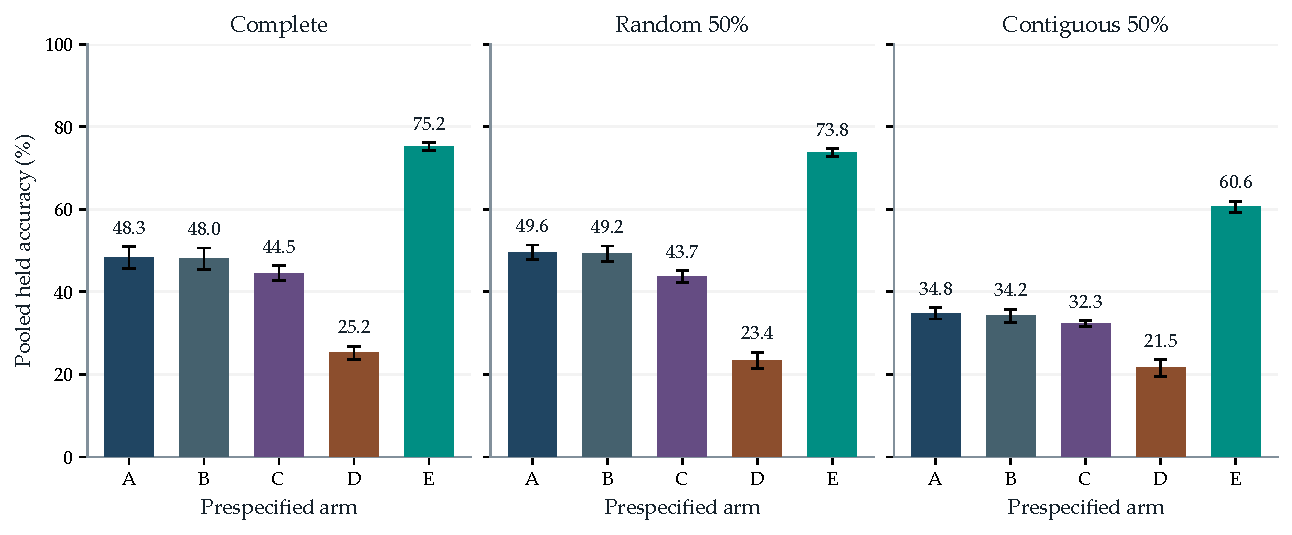
\includegraphics[width=.98\textwidth]{mira_v2_held_accuracy.pdf}
\caption{Every prespecified arm on pooled held recordings. Error bars are sample SD over five training seeds, after averaging masks within seed; they are not confidence intervals. Complete input uses one realization. Random and contiguous loss each remove 250 normalized positions shared by all channels. The feature-only arm E performs substantially better here than the hybrid arms; the plot retains the unsuccessful main candidate A and temporal control D.}
\label{fig:m2-held}
\end{figure*}
\begin{figure*}[t]
\centering
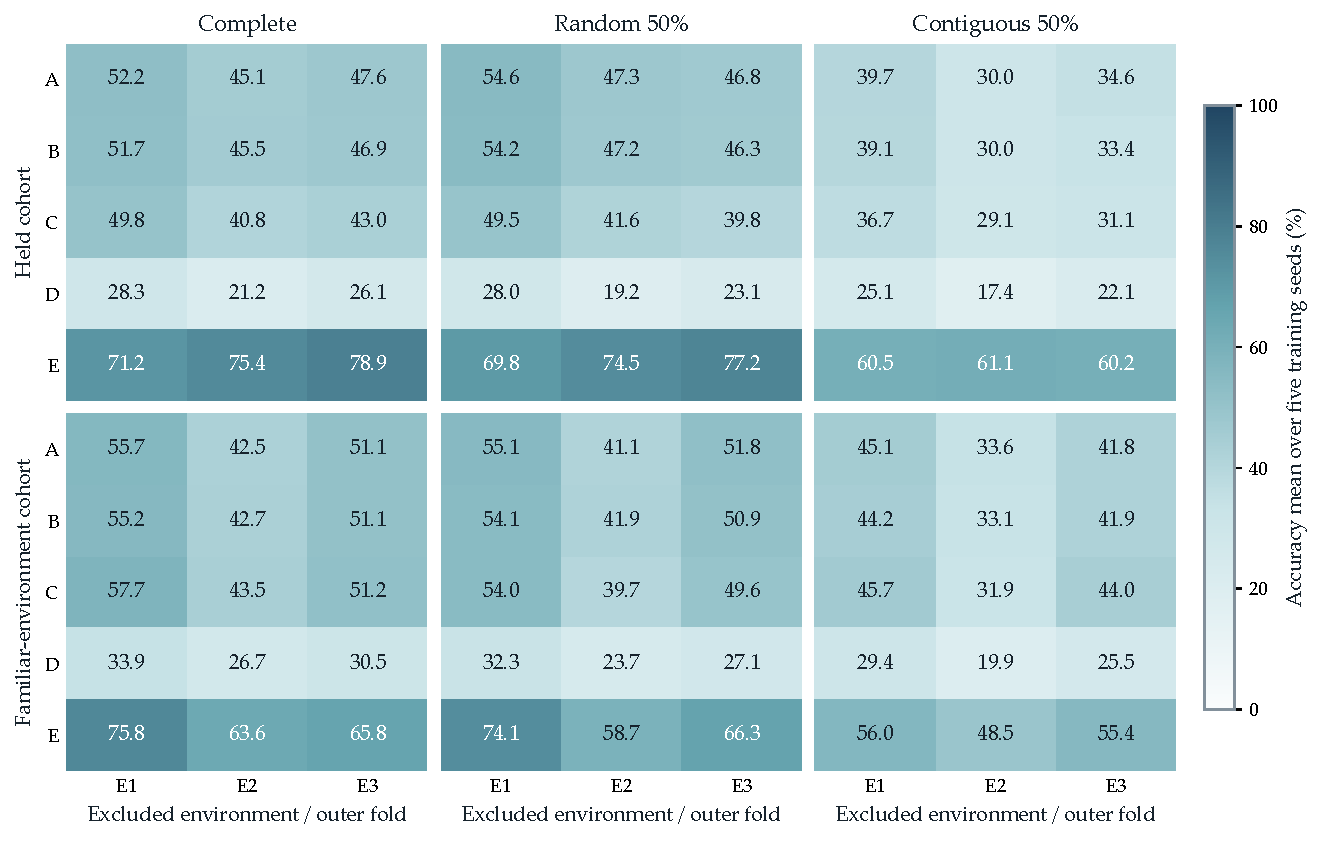
\includegraphics[width=.98\textwidth]{mira_v2_fold_domain_accuracy.pdf}
\caption{All arms, folds and cohort domains. Each cell shows mean accuracy across five training seeds after mask averaging, on a common 0--100\% colour scale. Top: the excluded environment/cohort; bottom: participants held out within the remaining two environments. E1--E3 always identify the excluded environment. Familiar and held scores are not mixed, and familiar scores are not consistently greater. Full sample SD, macro F1, NLL and Brier appear in Supplementary Tables S1--S6; Table~\ref{tab:m2-E} retains E's full 18-row breakdown in the main text.}
\label{fig:m2-folds}
\end{figure*}
\begin{figure*}[t]
\centering
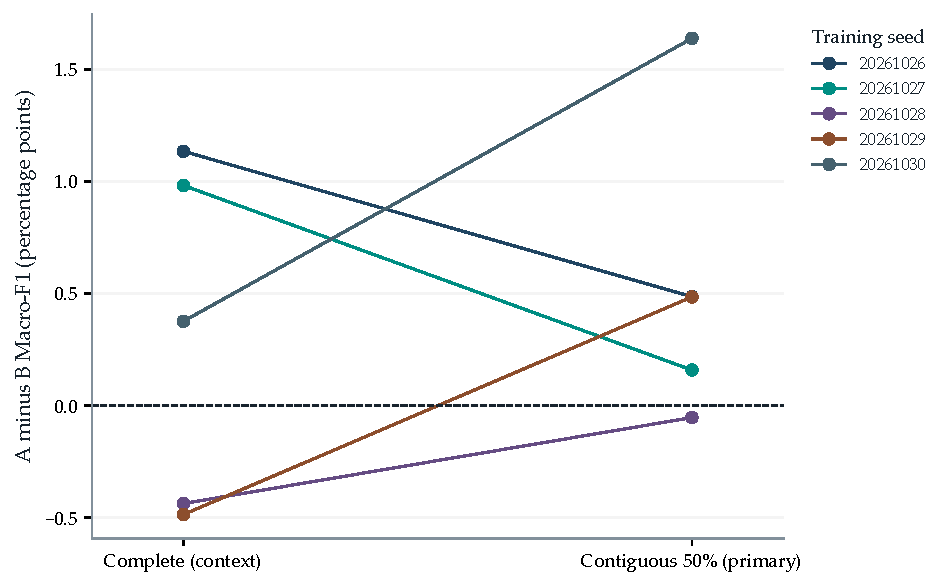
\includegraphics[width=.78\textwidth]{mira_v2_primary_paired_contrast.pdf}
\caption{Paired A minus B macro-F1 differences for each training seed. Loss-mask results are averaged before forming the five seed differences. The primary contiguous-loss contrast is $+0.543\pm0.654$ percentage points, with four positive and one negative seed difference. The clean differences are retained as context because A and B also differ on complete input. Lines join the same seed; they do not describe a physical trajectory or independent participant observations.}
\label{fig:m2-primary}
\end{figure*}


\subsection*{Interpretation, limitations and reproducibility}
The result most directly supports further investigation of a compact
fixed-feature classifier on this processed dataset. It does not validate
the original preference for the hybrid A. Since the feature-only counterpart
using B's denominator was not included, E's advantage over A--D does not
isolate support matching from the feature family, fusion, capacity or
optimization. Such a comparator and external data would require a separately
specified follow-up, not retrospective replacement of the current primary
comparison. We preserve A's weak result alongside E's encouraging result.

The source-selected MiniRocket study uses a different representation and
learning setup~\cite{dempster2021}. Its numbers and those of the present
extension do not form a controlled attribution of algorithmic superiority.
We therefore make no claim of beating MiniRocket generally, achieving
state-of-the-art performance, inventing known
covariance, masking, MLP or convolution components.

The fixed log-power floor, packet-index resampling, cell boundaries and
lags are part of the tested representation. Removing normalized positions
does not reproduce a raw timestamped acquisition outage, and observed
endpoints do not reconstruct missing movements between them. No experiment
here produces a human image, pose, temperature or vital sign, or validates
continuous live sensing. Rank truncation and padding constrain the feature-level
invariance, and the CNN has no general invariance guarantee. A possible
future source diagnostic of ranks or invalid cells must not become a
retrospective target-guided threshold search.

Input masks in the executed experiment are Boolean and the feature preparation
was checked for independence from hidden fills. A separate interface review
found that the preparation wrapper casts an externally supplied mask to
Boolean before validating it; non-binary or NaN external mask entries would
therefore be unsafe. This is a documented API precondition/limitation, not
evidence of hidden-value access in the present Boolean-mask run. The separate public prediction wrapper validates masks before conversion and rejects non-finite intermediate or output values. The archived implementation and the recorded experimental outputs remain unchanged.

The complete CPU source execution took 2,225.70 seconds; the separate
evaluation stage took 1,933.15 seconds on this machine with two compute
threads. These are execution wall times, including feature preparation and
output handling, not portable inference-latency benchmarks. Independent
source replay matched 12,600 validation probability vectors exactly; the
test-output audit checked 485,100 saved probability vectors and recomputed
1,650 per-fit/condition/domain metric rows without an additional model
forward or optimizer step. These counts include repeated views of fixed
recordings, not new samples. Five-seed summaries retain all 90
arm/fold/domain/condition combinations.

The representation cache, manifest, frozen source checkpoints, source
temperatures, saved test probabilities and report tables have SHA256 receipts.
The protocol hash begins \texttt{cc407a98f343}; the all-fit source freeze
begins \texttt{c7575d16aefd}. This audit establishes correspondence between
the declared execution and its reported numbers, not scientific priority,
absence of all implementation defects, or external validity. Because model
development followed historical target inspection and cohorts differ by
environment, a new independent dataset or prospectively untouched evaluation
is needed to assess reproducibility and generalization.

\subsection*{Additional MiniRocket reference on the fixed power18 input}
\label{sec:matched-p18}

To reduce the input-representation mismatch in the earlier comparison, we
added an official MiniRocket reference~\cite{dempster2021} on the same fixed
18-stream, 500-position log-mean-power input used by the spectral extension.
The reference retains the same participant roles, three outer folds, five
training seeds and test masks. Three previously fitted source configurations
were reused, and 12 further source fits completed the 15 fold/seed
configurations. These are 15 reference models, not 15 new datasets or an
additional selection among target scores. The source and evaluation freezes
and independent output checks bind the saved configurations and predictions.
No E weights were retrained for this comparison. The official multivariate MiniRocket transform uses 9,996 features (10,000 requested), maximum dilations per kernel 32, and separately reset NumPy and Numba random generators for each training seed. Transform parameters and a feature scaler with no centering are fitted only on the 504 source-training recordings; ridge regularization is fixed at $\alpha=1$. A scalar temperature in $[0.1,10]$ minimizes NLL only on the 168 clean source-validation recordings and is retained under loss.

The alignment is deliberately limited. E uses loss augmentation and
actual-mask features, whereas MiniRocket is clean-trained. At test time the
reference receives missing power18 entries filled with source-training band
means; it has no explicit mask or distance channel. The comparison therefore
aligns input representation and prediction roles, but not training policy,
loss treatment or classifier family. It is a useful additional reference,
not a controlled attribution of a difference to architecture or to support
matching. It was added after E's outcomes were known, so its status is
post-hoc and exploratory; it is not a new confirmation of the original
primary hypothesis or a state-of-the-art claim.

Table~\ref{tab:matched-p18} reports every complete, random-loss and
contiguous-loss condition for E, MiniRocket and the A/B hybrid controls,
including familiar-environment results. Metrics are calculated from saved
probabilities. For each training seed and loss-mask realization, held-fold
predictions are concatenated before calculating accuracy, seven-class macro
F1, NLL and summed multiclass Brier. Masks are then averaged within the
training seed; the displayed mean and sample SD are over five training
seeds. Complete input has one realization; each loss condition has five.
These SDs are not confidence intervals. The pooled familiar summary contains
504 fold-specific prediction occurrences, with possible repeat recordings
and participants across folds, rather than 504 independent new recordings.

\paragraph{Results and retained controls.}
E's pooled held accuracy is $75.175\pm1.005$\% on complete input, compared
with $53.841\pm0.938$\% for this MiniRocket reference. Under random 50\% loss,
the respective values are $73.822\pm0.942$\% and $22.305\pm1.102$\%;
under contiguous 50\% loss they are $60.597\pm1.375$\% and
$19.406\pm2.330$\%. Corresponding held macro F1 under contiguous loss is
$59.159\pm1.610$\% for E and $15.636\pm4.147$\% for the reference.
NLL is $1.160\pm0.014$ versus $4.852\pm1.764$, and Brier is
$0.552\pm0.011$ versus $1.275\pm0.168$, in that condition. This reference
degrades sharply under its declared mean-fill policy; the observation does
not establish that all MiniRocket training or repair configurations behave
similarly. Figure~\ref{fig:matched-p18} retains the full complete-to-loss
comparison on a common percentage scale.

The A/B hybrid controls remain weaker on complete held input than this
reference: their accuracies are $48.302\pm2.627$\% and
$48.048\pm2.559$\%, respectively. Thus the added reference does not reverse
the negative result for the main hybrid A. E also remains imperfect under
loss: its contiguous-loss macro F1 is below 60\%, and its pooled familiar
accuracy is $53.325\pm1.480$\% in that condition, compared with
$20.579\pm4.082$\% for MiniRocket. Familiar and held cohorts must not be
treated as an isolated causal room intervention.

\paragraph{Paired contrasts and conditional uncertainty.}
The additional E-minus-MiniRocket held macro-F1 contrast under contiguous
50\% loss is $+43.524\pm3.639$ percentage points across the five paired
training-seed differences, after mask averaging. All five seed differences
are positive. The reported 95\% conditional bootstrap range is
$[39.879,47.054]$ percentage points. For each of 10,000 paired bootstrap
draws (seed 20261028), ten participants are sampled with replacement from
the ten observed participants in each fixed environment. The same participant
multiplicities apply to both models, all five training seeds and all five
contiguous-loss masks. Weighted pooled confusion counts yield macro F1 for
each training-seed/mask cell, and the 25 cell contrasts are averaged.
This preserves pairing and repeated-view dependence. Environments, trained
models, training/mask seeds and the observed dataset remain fixed.
The range is descriptive and conditional: it does not represent uncertainty
over new rooms or training datasets and is not corrected for post-hoc
selection or multiple comparisons. No p-value or population-level
confirmation is inferred from its exclusion of zero.

The original A-minus-B primary comparison is kept separate. It remains
$+0.543\pm0.654$ macro-F1 percentage points under contiguous loss, with four
positive and one negative training-seed difference; its corresponding
descriptive conditional range is $[0.041,1.068]$ points. A--B changes
endpoint weighting, centering and covariance normalization even on complete
input. Both A and B share ideal full-effective-support congruence invariance,
and E's feature-only counterpart with B's denominator was not evaluated.
Consequently the large additional E--reference contrast does not isolate a
benefit caused by support matching, replace the small primary contrast, or
confirm its proposed mechanism. A training-policy-matched comparison and
independent data remain necessary for broader claims.

\begin{table*}[t]
\centering
\caption{Fixed-power-input comparison, retaining E, the clean-trained MiniRocket reference (MR-P18), and both hybrid controls. C: complete; R50/B50: random/contiguous 50\% loss. Values are mean $\pm$ sample SD across five training seeds after mask averaging, not confidence intervals. Accuracy and macro F1 are percentages; NLL and summed multiclass Brier are unitless. Held pools 1,260 recordings; familiar pools 504 fold-specific prediction occurrences, with possible repeated recordings/participants across folds. E is loss-augmented; MR-P18 is clean-trained with source-band-mean fill and no mask input, so this is not a training-policy-matched architectural comparison.}
\label{tab:matched-p18}
\begingroup\fontsize{9.5}{12}\selectfont
\setlength{\tabcolsep}{4pt}\renewcommand{\arraystretch}{1.13}
\setlength{\extrarowheight}{1.3pt}\setlength{\arrayrulewidth}{0.5pt}\arrayrulecolor{mrefBorder}
\begin{tabularx}{\textwidth}{|lll*{4}{>{\raggedleft\arraybackslash}X}|}
\hline\rowcolor{mrefHead}
\mrefHeadText{Model} & \mrefHeadText{Cohort} & \mrefHeadText{Input} & \mrefHeadText{Accuracy (\%)} & \mrefHeadText{Macro F1 (\%)} & \mrefHeadText{NLL} & \mrefHeadText{Brier} \\
\hline
\rowcolor{mrefE}
E & Held & C & 75.17\,\(\pm\)\,1.00 & 74.61\,\(\pm\)\,1.21 & 0.773\,\(\pm\)\,0.018 & 0.365\,\(\pm\)\,0.008 \\
\rowcolor{mrefE}
E & Held & R50 & 73.82\,\(\pm\)\,0.94 & 73.33\,\(\pm\)\,1.10 & 0.831\,\(\pm\)\,0.018 & 0.386\,\(\pm\)\,0.009 \\
\rowcolor{mrefE}
E & Held & B50 & 60.60\,\(\pm\)\,1.37 & 59.16\,\(\pm\)\,1.61 & 1.160\,\(\pm\)\,0.014 & 0.552\,\(\pm\)\,0.011 \\
\rowcolor{mrefE}
E & Familiar & C & 68.41\,\(\pm\)\,1.26 & 67.97\,\(\pm\)\,1.39 & 0.883\,\(\pm\)\,0.051 & 0.448\,\(\pm\)\,0.019 \\
\rowcolor{mrefE}
E & Familiar & R50 & 66.40\,\(\pm\)\,0.84 & 65.77\,\(\pm\)\,0.93 & 0.946\,\(\pm\)\,0.051 & 0.470\,\(\pm\)\,0.014 \\
\rowcolor{mrefE}
E & Familiar & B50 & 53.33\,\(\pm\)\,1.48 & 51.51\,\(\pm\)\,1.64 & 1.341\,\(\pm\)\,0.059 & 0.648\,\(\pm\)\,0.019 \\
\hline
\rowcolor{mrefMR}
MR-P18 & Held & C & 53.84\,\(\pm\)\,0.94 & 53.87\,\(\pm\)\,1.01 & 1.363\,\(\pm\)\,0.037 & 0.634\,\(\pm\)\,0.009 \\
\rowcolor{mrefMR}
MR-P18 & Held & R50 & 22.30\,\(\pm\)\,1.10 & 16.11\,\(\pm\)\,0.84 & 3.486\,\(\pm\)\,0.151 & 1.109\,\(\pm\)\,0.023 \\
\rowcolor{mrefMR}
MR-P18 & Held & B50 & 19.41\,\(\pm\)\,2.33 & 15.64\,\(\pm\)\,4.15 & 4.852\,\(\pm\)\,1.764 & 1.275\,\(\pm\)\,0.168 \\
\rowcolor{mrefMR}
MR-P18 & Familiar & C & 58.85\,\(\pm\)\,0.57 & 58.30\,\(\pm\)\,0.77 & 1.295\,\(\pm\)\,0.043 & 0.588\,\(\pm\)\,0.010 \\
\rowcolor{mrefMR}
MR-P18 & Familiar & R50 & 22.38\,\(\pm\)\,1.37 & 15.84\,\(\pm\)\,1.40 & 3.388\,\(\pm\)\,0.282 & 1.105\,\(\pm\)\,0.043 \\
\rowcolor{mrefMR}
MR-P18 & Familiar & B50 & 20.58\,\(\pm\)\,4.08 & 16.75\,\(\pm\)\,5.85 & 4.812\,\(\pm\)\,1.797 & 1.263\,\(\pm\)\,0.194 \\
\hline
\rowcolor{mrefA}
A & Held & C & 48.30\,\(\pm\)\,2.63 & 47.55\,\(\pm\)\,2.93 & 1.395\,\(\pm\)\,0.052 & 0.690\,\(\pm\)\,0.028 \\
\rowcolor{mrefA}
A & Held & R50 & 49.58\,\(\pm\)\,1.76 & 49.15\,\(\pm\)\,1.99 & 1.327\,\(\pm\)\,0.032 & 0.665\,\(\pm\)\,0.024 \\
\rowcolor{mrefA}
A & Held & B50 & 34.77\,\(\pm\)\,1.37 & 34.04\,\(\pm\)\,1.38 & 2.127\,\(\pm\)\,0.084 & 0.902\,\(\pm\)\,0.021 \\
\rowcolor{mrefA}
A & Familiar & C & 49.76\,\(\pm\)\,1.86 & 48.59\,\(\pm\)\,1.62 & 1.402\,\(\pm\)\,0.061 & 0.677\,\(\pm\)\,0.020 \\
\rowcolor{mrefA}
A & Familiar & R50 & 49.33\,\(\pm\)\,0.45 & 48.39\,\(\pm\)\,0.48 & 1.352\,\(\pm\)\,0.029 & 0.660\,\(\pm\)\,0.009 \\
\rowcolor{mrefA}
A & Familiar & B50 & 40.16\,\(\pm\)\,1.30 & 39.46\,\(\pm\)\,1.05 & 1.904\,\(\pm\)\,0.072 & 0.822\,\(\pm\)\,0.012 \\
\hline
\rowcolor{mrefB}
B & Held & C & 48.05\,\(\pm\)\,2.56 & 47.24\,\(\pm\)\,2.78 & 1.412\,\(\pm\)\,0.046 & 0.696\,\(\pm\)\,0.029 \\
\rowcolor{mrefB}
B & Held & R50 & 49.23\,\(\pm\)\,1.89 & 48.48\,\(\pm\)\,2.19 & 1.361\,\(\pm\)\,0.040 & 0.673\,\(\pm\)\,0.029 \\
\rowcolor{mrefB}
B & Held & B50 & 34.19\,\(\pm\)\,1.60 & 33.49\,\(\pm\)\,1.56 & 2.143\,\(\pm\)\,0.083 & 0.908\,\(\pm\)\,0.021 \\
\rowcolor{mrefB}
B & Familiar & C & 49.68\,\(\pm\)\,1.36 & 48.67\,\(\pm\)\,1.11 & 1.413\,\(\pm\)\,0.056 & 0.681\,\(\pm\)\,0.016 \\
\rowcolor{mrefB}
B & Familiar & R50 & 48.98\,\(\pm\)\,0.87 & 48.08\,\(\pm\)\,0.26 & 1.364\,\(\pm\)\,0.030 & 0.665\,\(\pm\)\,0.008 \\
\rowcolor{mrefB}
B & Familiar & B50 & 39.73\,\(\pm\)\,1.35 & 39.31\,\(\pm\)\,0.96 & 1.930\,\(\pm\)\,0.060 & 0.831\,\(\pm\)\,0.015 \\
\hline
\end{tabularx}
\arrayrulecolor{black}\endgroup
\end{table*}

\begin{figure*}[t]
\centering
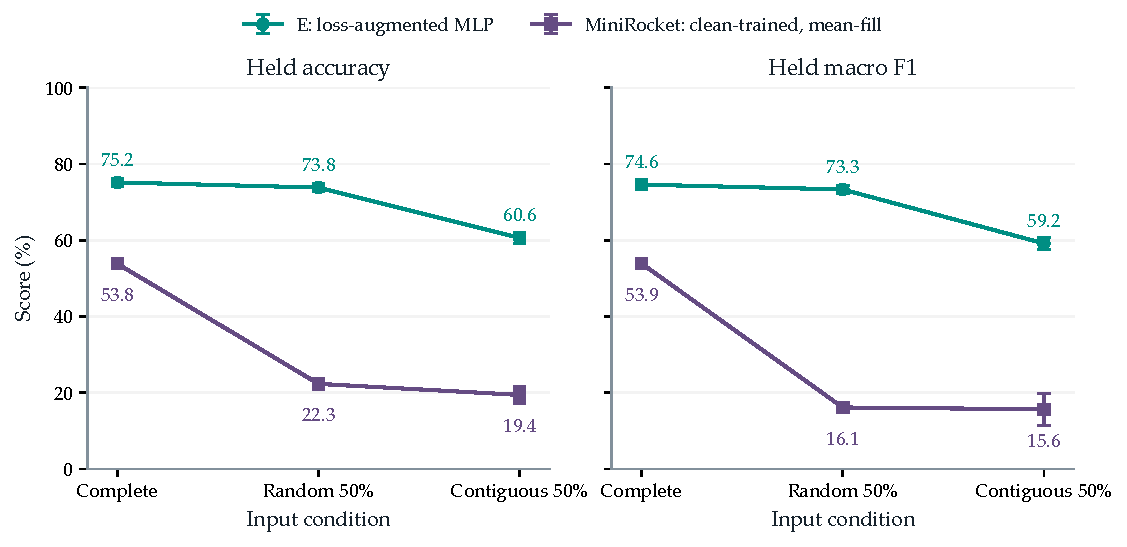
\includegraphics[width=.98\textwidth]{matched_power18_comparison.pdf}
\caption{Post-hoc comparison on the same fixed power18 representation and held prediction roles. Error bars are sample SD over five training seeds after within-seed mask averaging. The E--reference difference includes training and loss-treatment differences: E uses loss augmentation and actual-mask features; MiniRocket is clean-trained and receives source-band-mean-filled input without a mask. These curves do not isolate an architectural or support-matching effect and are not an independent confirmation or a state-of-the-art ranking. A/B controls and familiar results remain in Table~\ref{tab:matched-p18}.}
\label{fig:matched-p18}
\end{figure*}



\section{Discussion}
The completed comparisons show why model capacity, missingness handling and transfer must be assessed separately. Among the original mean-log-amplitude models, MiniRocket has stronger clean recognition, but its long-gap probability errors are larger in the original-representation loss experiment. Source-selected recording normalization improves its clean accuracy, without testing its loss robustness. Residual capacity improves on the compact CNNs in that mean-log-amplitude follow-up. The separate log-mean-power extension changes the empirical picture: its feature-only arm E reaches 75.17\% complete and 60.60\% contiguous-loss accuracy, whereas its hybrid A remains at 48.30\% and 34.77\%. Those are outcomes for distinct specified pipelines; the higher E score does not identify a unique cause or validate every proposed component. The additional fixed-power MiniRocket reference reaches 53.84\% complete and 19.41\% contiguous-loss accuracy, while using clean source training and dense source-mean filling. The difference from E is a comparison of specified pipelines, not an isolated architectural or augmentation effect. These results cannot support a claim that high-capacity deep learning universally fails after achieving high source accuracy. All transfer statements use within-dataset partitions.

Structured loss changes information before the classifier sees it. A long interpolated gap is determined by its observed boundary samples; it cannot uniquely recover an unobserved transition. The feature set includes temporal-bin means and first-difference statistics, both affected by that operation. This gives a plausible processing explanation for degradation, but a causal account of the individual class failures requires feature-specific ablations and further controlled acquisition. The original mean-log-amplitude extension compares three fixed repair operators but does not isolate every representation effect. These experiments do not establish that all CSI representations respond in the same way.

The interaction results also refine the original hypothesis. Additional error under loss is not consistently larger in the target domain. Low clean accuracy leaves different scope for further error, and cohort and class-specific confusions can alter the contrast. Reporting both signs is necessary; selecting only the positive cells would overstate the evidence. Future comparisons should include additional frozen baselines and independently collected environments before generalizing this pattern.

Target-data access defines a separate comparison axis. Standard domain-adversarial training uses labelled source observations and unlabelled target observations \cite{ganin2016}. Such a method would require an explicitly separate adaptation protocol here, because the present fitting and calibration exclude target observations. An adversarial alignment restricted to the source environments could preserve that access constraint, but it has not been evaluated in this study. Neither access to target data nor an adaptation method constitutes a guaranteed performance upper bound.

The component-removal follow-up constrains the model contribution more directly than a bundled CNN/MIRA comparison. Under the declared block-loss procedure, the explicit mask-input contrast is inconclusive, the distance input has a small adverse classification association relative to its removal control, and the coverage-pooling contrast does not exclude zero after the three-comparison adjustment. These are useful design findings rather than evidence that every proposed component must help. The analysis is conditional on this training procedure and dataset; it neither proves universal component failure nor isolates a physical cause. Learned CSI recovery methods offer additional comparisons \cite{zhao2024csibert,zhao2026csibert2}, but their training access, reconstruction objectives and tasks must be matched before importing performance claims.

The augmented residual control also scores below its clean-trained counterpart in the reported complete, random-loss and block-loss conditions. This observation does not identify a cause. The training distribution mixes clean views with several loss fractions and repairs, whereas checkpoint selection minimizes clean source-validation NLL. In the declared sampling scheme, contiguous 50\% loss has probability $1/12$ per training view, or $1/36$ with a particular repair. A mismatch between that mixture, the selection objective and the evaluated condition is a plausible hypothesis, not an experimentally isolated explanation. Mean repair can also introduce constant interiors and boundary changes, but the present comparison does not attribute the performance difference to those features. Testing these hypotheses would require source-selected augmentation and checkpoint-objective controls with a separate frozen evaluation.

Calibration and rejection require their own validation. NLL and Brier scores worsened under block loss despite a temperature fitted only to clean source validation. Saved selective-error metrics use 134/168 accepted familiar files (79.76\%) and 336/420 target files (80\%), ranked separately within condition. Such ranking describes a risk--coverage relationship; it does not produce a threshold guaranteed to control error on a new site. Deployment would require a separate validation protocol and a frozen operating rule.

The scope remains activity classification. Conceptual body meshes, colored wavefronts, and water-content diagrams explain concepts; none is a measured pose, temperature map, RF solution or physiological estimate. Inputs are presegmented, single-activity recordings with known boundaries. Continuous-stream detection and unseen activities are not evaluated. Different cohorts per environment also prevent separating room and person effects. It does not validate unrestricted sensing in homes, universities, companies, or multi-person scenes.

\section{Reproducibility and conclusion}
The source revision, file hashes, participant roles, trial IDs, mask seeds, model settings, temperatures, probability vectors, score tables, and bootstrap indices are retained. Independent calculations reproduced all 372 transfer metric rows from 109,368 predictions; all 1,260 input SHA256 hashes were rechecked. Radio scaling was independently spot-checked on nine files. These checks do not validate unrecorded acquisition conditions or original labels.

The package contains executable analyses and numerical outputs; recordings remain linked to the public sources \cite{alsaify2020,multienvdata}. The earlier NTU-Fi loss-only pilot appears in Appendix~\ref{app:ntu}, uses a different dataset and label set, and is not pooled with the main study. The MIRA-CSI software, model card and citation metadata are publicly available at \href{https://github.com/ABDESSAMAD-BOURKIBATE/mira-csi}{the author repository} \cite{bourkibate2026mira}. This secondary analysis involved no new participant recruitment or sensing hardware.

The initial extension and follow-up retain separate frozen protocols and outputs. The latter contributes 90 checkpoint-verified fits, 5,580 independently reconstructed metric rows and 1,640,520 saved probability vectors; its source-only archive is preserved separately from target evaluation. The representation sensitivity contributes 30 sealed fit configurations and 12,600 independently checked clean held predictions, with explicit reuse of previously fitted seed-one models. These counts describe computational artifacts and repeated evaluations, not an increase in the 30-participant sample. Script versions, input and prediction hashes, exact masks and participant-bootstrap draws accompany the corresponding result packages.

The spectral extension adds 75 source-fitted and checkpoint-verified models, 485,100 saved test probability vectors and 1,650 independently reconstructed condition/domain rows. These are repeated evaluations of the same recordings, not additional participants. Its primary hybrid A--B difference is small and changes direction across training seeds. The prespecified feature-only E comparator is substantially stronger within this execution, with mean accuracy of 75.17\% complete, 73.82\% random-loss and 60.60\% contiguous-loss, but its prominence is an exploratory outcome after historical target inspection. It does not prove support matching, causal room invariance or general algorithmic superiority. The additional 15-configuration fixed-power MiniRocket comparison, including three reused source fits, retains 97,020 saved probability vectors and 330 reconstructed domain/condition rows. E outperforms this fixed reference, but differences in training policy and loss treatment prevent attributing that advantage to architecture alone. Across the studies, recognition, component effects, input representation and probability quality require separate reporting. Independent replication with matched participants across more rooms and deployment-relevant acquisition remains necessary.


\appendix
\section{Separate NTU-Fi pipeline pilot}\label{app:ntu}
A prespecified subset of NTU-Fi HAR exercises the loss-only evaluation. This pilot uses the released train/test partition and does not evaluate held-out environments.

\begin{figure*}[t]
\centering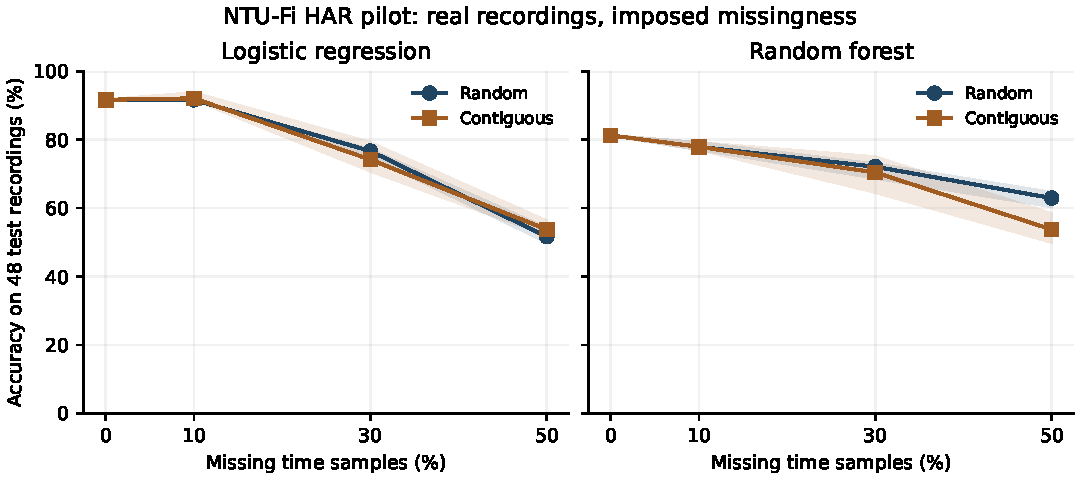
\includegraphics[width=\textwidth]{loss_accuracy.pdf}
\caption{Computed pilot accuracy on the same 48 test recordings after linear interpolation. Lines average five mask realizations; shading spans their minimum and maximum. This band measures mask variability, not a confidence interval. These curves derive from genuine recordings and are separate from the explanatory 3D illustrations.}
\label{fig:pilotloss}
\end{figure*}

The SenseFi public archive \cite{yang2023} contains 936 training and 264 test files, with six activity classes. A fixed SHA256 ranking selected 12 training, four validation, and eight test files per class: 72/24/48 files in total. Validation came exclusively from the released training partition. File checks found no non-finite values or exact duplicates in the selected inputs. Subject, session, and room identifiers were unavailable in this processed release.

Each file provides a 342-by-2000 amplitude array. Following the released loader, every fourth time sample was retained. Three antenna streams were summarized over six subcarrier bands using six statistics and ten temporal-bin means, yielding 288 features. Logistic regression ($C=1$; training-only standardization) and a 200-tree random forest (minimum leaf size two) were fitted once. Temperature scaling used only the 24 clean validation files.

At each loss fraction, exactly 50, 150, or 250 of 500 time positions were masked across all channels. Uniform random masks and one contiguous block were generated with five fixed seeds. Linear interpolation used observed values only, with held boundary values. Test labels did not influence model fitting, calibration, or mask generation.

\begin{center}
\begin{minipage}{\columnwidth}
\refstepcounter{table}\label{tab:pilot}
{\fontsize{9.3}{12}\selectfont\textbf{Table~\thetable.} Pilot accuracy (\%). LR: logistic regression; RF: random forest. Corrupted conditions average five masks on the same 48 files.\par}
\vspace{5pt}
\begingroup
\sffamily\fontsize{9.2}{12}\selectfont
\setlength{\tabcolsep}{5pt}
\renewcommand{\arraystretch}{1.45}
\begin{tabularx}{\linewidth}{>{\raggedright\arraybackslash}p{.43\linewidth}*{2}{>{\centering\arraybackslash}X}}
\rowcolor{foresthead}\multicolumn{1}{l}{\textcolor{white}{\bfseries Input condition}} & \multicolumn{1}{c}{\textcolor{white}{\bfseries LR}} & \multicolumn{1}{c}{\textcolor{white}{\bfseries RF}}\\
\rowcolor{mintfill}Complete & 91.7 & 81.3\\
\rowcolor{referencefill}Random 10\% & 91.7 & 77.9\\
\rowcolor{referencefill}Random 30\% & 76.7 & 72.1\\
\rowcolor{referencefill}Random 50\% & 51.7 & 62.9\\
\rowcolor{jointfill}Block 10\% & 92.1 & 77.9\\
\rowcolor{jointfill}Block 30\% & 74.2 & 70.4\\
\rowcolor{jointfill}Block 50\% & 53.8 & 53.8\\
\end{tabularx}
\endgroup
\end{minipage}
\end{center}


Complete-input accuracy was 44/48 (91.7\%) for logistic regression and 39/48 (81.3\%) for the forest. At 50\% contiguous loss, both averaged 53.8\%, whereas random loss gave 51.7\% and 62.9\%, respectively. The loss-pattern ordering therefore depended on the classifier in this subset; the pilot does not establish a universal ordering.

After clean-validation calibration, mean negative log-likelihood increased from 0.162 to 3.636 for logistic regression and from 0.404 to 1.457 for the forest under 50\% contiguous loss. Thus, equal accuracy can coexist with different probability errors. Risk--coverage values and per-file predictions are retained for further analysis.

These are descriptive results for one small, fixed subset. Five masks are repeated corruptions of the same files, not five independent datasets. Unavailable participant and session identifiers prevent stronger independence checks. The main transfer experiment uses a separately documented dataset; the pilot scores are not cross-environment results and are not pooled with that experiment.




\begin{figure*}[t]
\centering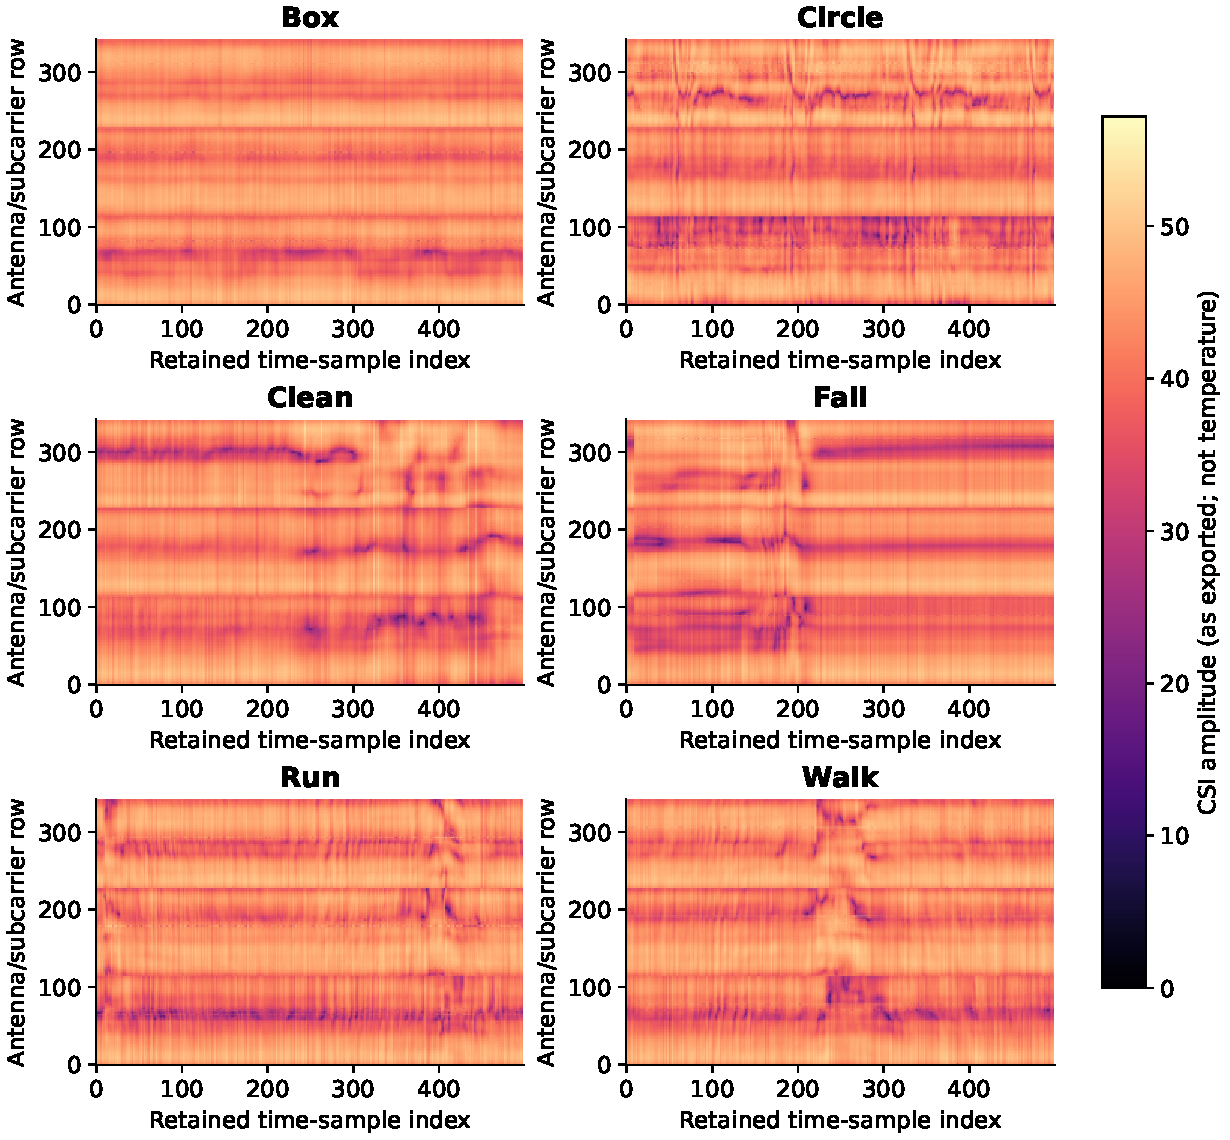
\includegraphics[width=\textwidth]{csi_activity_maps.pdf}
\caption{Genuine CSI amplitude examples for six activities. Each panel uses the lexically first selected training file of that class, with every fourth time sample retained. All panels share a color scale in the original exported amplitude units, without interpreting it as calibrated power or temperature. The horizontal coordinate is sample index, not elapsed seconds. The vertical coordinate stacks three antenna links and their 114 subcarriers.}
\label{fig:csimaps}
\end{figure*}

Figure~\ref{fig:csimaps} contains genuine six-class NTU-Fi pilot inputs on their original exported amplitude scale. These examples, the 48-file pilot scores and its unavailable participant metadata remain separate from the seven-label, participant-disjoint main study. The full pilot manifests and saved predictions remain in the supplementary reproduction archive.

\begingroup
\fontsize{9.5}{12.5}\selectfont
\noindent\textbf{Declarations.} No specific funding was received for this study. The author declares no relevant financial or non-financial competing interests, including through Share'In Holding. This analysis reuses public data; no new participants were recruited.

\noindent\textbf{Use of AI-assisted tools.} AI-based tools assisted manuscript drafting, software development and preparation of explanatory illustrations. Quantitative results were computed from the documented public recordings and checked against saved predictions through separate verification procedures. The author is responsible for reviewing and approving the final manuscript, code, references and figures.
\par\endgroup

% Finish all pending figures before the final references section.
\onecolumn
\begingroup
\begin{multicols}{2}
\fontsize{9}{11.3}\selectfont



\renewcommand{\bibfont}{\normalfont\fontsize{9}{11.3}\selectfont}
\setlength{\bibsep}{3pt}
\begin{thebibliography}{17}
\raggedright
\interlinepenalty=10000
\bibitem{zinys2021}
A. Zinys, B. van Berlo, and N. Meratnia. A Domain-Independent Generative Adversarial Network for Activity Recognition Using WiFi CSI Data. \textit{Sensors}, 21(23):7852, 2021. \href{https://doi.org/10.3390/s21237852}{\nolinkurl{doi:10.3390/s21237852}}.
\bibitem{guarino2026}
I. Guarino, D. Carra, M. Cominelli, F. Gringoli, and R. Lo Cigno. A survey on CSI-based Wi-Fi sensing datasets and models with a focus on reproducibility. \textit{Computer Communications}, 249:108431, 2026. \href{https://doi.org/10.1016/j.comcom.2026.108431}{\nolinkurl{doi:10.1016/j.comcom.2026.108431}}.
\bibitem{geng2022}
J. Geng, D. Huang, and F. De la Torre. DensePose From WiFi. \textit{arXiv preprint}, arXiv:2301.00250, submitted 31 December 2022. \href{https://doi.org/10.48550/arXiv.2301.00250}{\nolinkurl{doi:10.48550/arXiv.2301.00250}}.
\bibitem{zheng2019}
Y. Zheng, Y. Zhang, K. Qian, G. Zhang, Y. Liu, C. Wu, and Z. Yang. Zero-Effort Cross-Domain Gesture Recognition with Wi-Fi. In \textit{ACM MobiSys}, pp. 313--325, 2019. \href{https://doi.org/10.1145/3307334.3326081}{\nolinkurl{doi:10.1145/3307334.3326081}}.
\bibitem{yang2023}
J. Yang, X. Chen, H. Zou, C. X. Lu, D. Wang, S. Sun, and L. Xie. SenseFi: A library and benchmark on deep-learning-empowered WiFi human sensing. \textit{Patterns}, 4(3):100703, 2023. \href{https://doi.org/10.1016/j.patter.2023.100703}{\nolinkurl{doi:10.1016/j.patter.2023.100703}}.
\bibitem{guo2017}
C. Guo, G. Pleiss, Y. Sun, and K. Q. Weinberger. On Calibration of Modern Neural Networks. In \textit{ICML}, PMLR 70, pp. 1321--1330, 2017. \href{https://proceedings.mlr.press/v70/guo17a.html}{proceedings.mlr.press/v70/guo17a}.
\bibitem{geifman2017}
Y. Geifman and R. El-Yaniv. Selective Classification for Deep Neural Networks. In \textit{Advances in Neural Information Processing Systems}, vol. 30, 2017. \href{https://papers.nips.cc/paper_files/paper/2017/hash/4a8423d5e91fda00bb7e46540e2b0cf1-Abstract.html}{Official proceedings}.
\bibitem{alsaify2020}
B. A. Alsaify, M. M. Almazari, R. Alazrai, and M. I. Daoud. A dataset for Wi-Fi-based human activity recognition in line-of-sight and non-line-of-sight indoor environments. \textit{Data in Brief}, 33:106534, 2020. \href{https://doi.org/10.1016/j.dib.2020.106534}{\nolinkurl{doi:10.1016/j.dib.2020.106534}}.
\bibitem{multienvdata}
B. A. Alsaify, M. M. Almazari, R. Alazrai, and M. I. Aldaoud. A dataset for Wi-Fi-based human activity recognition in line-of-sight and non-line-of-sight indoor environments, v2. \textit{Mendeley Data}, 2021. \href{https://doi.org/10.17632/v38wjmz6f6.2}{\nolinkurl{doi:10.17632/v38wjmz6f6.2}}. Parsed MAT files and scaling code: \href{https://github.com/lcsig/Dataset-for-Wi-Fi-based-human-activity-recognition-in-LOS-and-NLOS-indoor-environments/tree/5337147c5156948b13e6b05a50b79529614acfbe}{author repository, pinned revision}.
\bibitem{halperin2011}
D. Halperin, W. Hu, A. Sheth, and D. Wetherall. Tool release: Gathering 802.11n traces with channel state information. \textit{ACM SIGCOMM Computer Communication Review}, 41(1):53, 2011. \href{https://doi.org/10.1145/1925861.1925870}{\nolinkurl{doi:10.1145/1925861.1925870}}.
\bibitem{usgs2019}
U.S. Geological Survey, Water Science School. The Water in You: Water and the Human Body. 22 May 2019. \href{https://www.usgs.gov/water-science-school/science/water-you-water-and-human-body}{USGS educational source}. Accessed 26 October 2026.
\bibitem{gabriel1996}
C. Gabriel and S. Gabriel. Compilation of the dielectric properties of body tissues at RF and microwave frequencies. Report AL/OE-TR-1996-0037, Armstrong Laboratory, Brooks Air Force Base, June 1996. \href{https://niremf.ifac.cnr.it/docs/DIELECTRIC/home.html}{Public report and data}.
\bibitem{espressif2026}
Espressif Systems. Wi-Fi Channel State Information Configure. \textit{ESP-IDF Programming Guide}, v6.1, ESP32. \href{https://docs.espressif.com/projects/esp-idf/en/v6.1/esp32/api-guides/wifi-driver/wifi-vendor-features.html}{Official documentation}. Accessed 26 October 2026.
\bibitem{efron1979}
B. Efron. Bootstrap Methods: Another Look at the Jackknife. \textit{The Annals of Statistics}, 7(1):1--26, 1979. \href{https://doi.org/10.1214/aos/1176344552}{\nolinkurl{doi:10.1214/aos/1176344552}}.
\bibitem{dempster2021}
A. Dempster, D. F. Schmidt, and G. I. Webb. MiniRocket: A Very Fast (Almost) Deterministic Transform for Time Series Classification. In \textit{ACM SIGKDD}, pp. 248--257, 2021. \href{https://doi.org/10.1145/3447548.3467231}{\nolinkurl{doi:10.1145/3447548.3467231}}. Basic multivariate reference code: \href{https://github.com/angus924/minirocket/tree/0b1c245d9c9dbc50886f28bc7b32d5d45b5663d6}{pinned source revision}.
\bibitem{che2018}
Z. Che, S. Purushotham, K. Cho, D. Sontag, and Y. Liu. Recurrent Neural Networks for Multivariate Time Series with Missing Values. \textit{Scientific Reports}, 8:6085, 2018. \href{https://doi.org/10.1038/s41598-018-24271-9}{\nolinkurl{doi:10.1038/s41598-018-24271-9}}.
\bibitem{ganin2016}
Y. Ganin, E. Ustinova, H. Ajakan, P. Germain, H. Larochelle, F. Laviolette, M. Marchand, and V. Lempitsky. Domain-Adversarial Training of Neural Networks. \textit{Journal of Machine Learning Research}, 17(59):1--35, 2016. \href{https://jmlr.org/papers/v17/15-239.html}{Official article and full text}.
\bibitem{zhao2024csibert}
Z. Zhao, T. Chen, F. Meng, H. Li, X. Li, and G. Zhu. Finding the Missing Data: A BERT-Inspired Approach Against Package Loss in Wireless Sensing. In \textit{IEEE INFOCOM 2024 -- IEEE Conference on Computer Communications Workshops (INFOCOM WKSHPS)}, pp. 1--6, 2024. \href{https://doi.org/10.1109/INFOCOMWKSHPS61880.2024.10620769}{\nolinkurl{doi:10.1109/INFOCOMWKSHPS61880.2024.10620769}}.
\bibitem{zhao2026csibert2}
Z. Zhao, F. Meng, Z. Lyu, H. Li, X. Li, and G. Zhu. CSI-BERT2: A BERT-Inspired Framework for Efficient CSI Prediction and Classification in Wireless Communication and Sensing. \textit{IEEE Transactions on Mobile Computing}, 25(5):7241--7257, 2026. \href{https://doi.org/10.1109/TMC.2025.3640420}{\nolinkurl{doi:10.1109/TMC.2025.3640420}}.
\bibitem{zakeri2026age}
A. Zakeri, N. T. Nguyen, and M. Juntti. Resource-Efficient Wi-Fi CSI-Based Sensing via Exploiting the Age of Samples. \textit{arXiv preprint}, arXiv:2606.31690v2, revised 5 October 2026. \href{https://doi.org/10.48550/arXiv.2606.31690}{\nolinkurl{doi:10.48550/arXiv.2606.31690}}.
\bibitem{bourkibate2026mira}
A. Bourkibate. MIRA-CSI: Missingness-Informed Recognition of Activities from Wi-Fi CSI. Software v0.1.0, 2026. \href{https://github.com/ABDESSAMAD-BOURKIBATE/mira-csi/releases/tag/v0.1.0}{Code, model states and evaluated release}. Experimental software; no DOI assigned.
\bibitem{m2pads}
K. Qian, C. Wu, Z. Yang, Y. Liu, and Z. Zhou.
PADS: Passive detection of moving targets with dynamic speed using PHY layer
information. In \textit{2014 20th IEEE International Conference on Parallel
and Distributed Systems (ICPADS)}, 2014.
\href{https://doi.org/10.1109/PADSW.2014.7097784}{doi:10.1109/PADSW.2014.7097784}.

\bibitem{m2sfa}
L. Wiskott and T. J. Sejnowski.
Slow feature analysis: Unsupervised learning of invariances.
\textit{Neural Computation}, 14(4):715--770, 2002.
\href{https://doi.org/10.1162/089976602317318938}{doi:10.1162/089976602317318938}.

\bibitem{m2sobi}
A. Belouchrani, K. Abed-Meraim, J.-F. Cardoso, and E. Moulines.
A blind source separation technique using second-order statistics.
\textit{IEEE Transactions on Signal Processing}, 45(2):434--444, 1997.
\href{https://doi.org/10.1109/78.554307}{doi:10.1109/78.554307}.

\bibitem{m2partial}
G. Liu, F. A. Reda, K. J. Shih, T.-C. Wang, A. Tao, and B. Catanzaro.
Image inpainting for irregular holes using partial convolutions.
In \textit{European Conference on Computer Vision (ECCV)}, pp. 85--100, 2018.
\href{https://www.ecva.net/papers/eccv_2018/papers_ECCV/html/Guilin_Liu_Image_Inpainting_for_ECCV_2018_paper.php}{Official proceedings}.
\end{thebibliography}
\end{multicols}
\endgroup
\end{document}
